\documentclass{article}
\usepackage[margin=1.0in]{geometry}
\usepackage{setspace}
\usepackage{tgschola}
\usepackage[T1]{fontenc}


\usepackage{indentfirst}
\usepackage{fancyhdr}
\usepackage{titlesec}
\usepackage{titletoc}

\usepackage{index}
\usepackage[columns=1]{idxlayout}

\usepackage{pdfpages}

\usepackage{hyperref}
\usepackage[font=Large]{caption}


\newindex{case}{cdx}{cnd}{Cases}
\newindex{statute}{sdx}{snd}{Statutes}

% COMMANDS TO GET INDICES TO COMPILE:
% makeindex -s toa.ist -o brief.snd brief.sdx 
% makeindex -s toa.ist -o brief.cnd brief.cdx

\hyphenation{re-search-ers}
\hyphenation{a-ca-dem-ia}

\date{\today}
\begin{document}
	
	\fontsize{14}{17}
	\selectfont
	  
	\titlecontents{section}
	    {}
	    {\normalsize \textsc}
	    {\hspace*{-2.3em}}
	    {\titlerule*[1pc]{.}\contentspage}
	

	\pagenumbering{roman}
	\thispagestyle{empty} % Gets rid of page number on the title page
	\begin{center}
		
		No. 13-1816
		
		\linethickness{0.5mm}
		\line(1,0){450}
		\vspace{-0.9em}
		\linethickness{0.25mm}
		\line(1,0){450}
		\vspace{0.20in}
		
		\textsc{In the United States Court of Appeals for the Third Circuit}
		\vspace{0.20in}
		
		\line(1,0){150}
		
		\vspace{0.20in}
		\textsc{United States of America,}
		\vspace{0.20in}
		\emph{Plaintiff-Appellee,}
		\vspace{0.05in}
		
		v.
		
		\vspace{0.20in}
		\textsc{Andrew Auernheimer,}
		\vspace{0.20in}
		\emph{Defendant-Appellant.}
		
		\line(1,0){150}
		
		\vspace{0.20in}
		Appeals from the United States District Court for the District of New Jersey, Case No. 11-CR-470, Judge Susan D. Wigenton
		\vspace{0.20in}
		
		\line(1,0){150}
		
		\vspace{0.20in}
		\textsc{Brief of Meredith Patterson, Brendan O'Connor, Sergey Bratus, Gabriella Coleman, Peyton Engel, Matthew Green, Dan Hirsch, Dan Kaminsky, Samuel Liles, Shane MacDougall, Brian Martin, C.\ Thomas, and Peiter Zatko as Amici Curiae Supporting Appellant}
		\vspace{0.20in}
		
		\line(1,0){150}
		
		\vspace{0.20in}
		\textsc{Alex Muentz} \\
		Adjunct Instructor \\
		Department of Criminal Justice \\
		Gladfelter Hall, 5th floor \\
		Temple University \\ 
		1115 Polett Walk \\
		Philadelphia PA 19122 \\
		(215) 806-4383 \\
		\vspace{0.20in}

		
		\line(1,0){450}
		\vspace{-0.9em}
		\linethickness{0.5mm}
		\line(1,0){450}		
		\linethickness{0.25mm} %Just so if we want a normal line later, we'll have it
		
	\end{center}
	
	\newpage
	
	\pagestyle{fancy}
	\fancyhead{}
	\fancyfoot{}
	\renewcommand{\headrulewidth}{0pt}
	\renewcommand{\footrulewidth}{0pt}
	\fancyfoot[C]{\fontsize{14}{17}\selectfont\thepage}
		
	\titleformat{\section}
		{\normalfont\Large}
		{}{1em}{\centering \textsc}
        
	\titlecontents{section}
	    {}
	    {\normalfont\Large \textsc}
	    {\hspace*{-2.3em}}
	    {\titlerule*[1pc]{.}\contentspage}
        
    \renewcommand{\thesubsection}{\arabic{subsection}} % This redefinition suppresses the section number, which we don't use
	\titleformat{\subsection}
		{\normalfont\Large}
		{\thesubsection.}{1em}{\textsc}
        
	\titlecontents{subsection}[2em]
	    {\normalfont\large \contentslabel{1em}}%{ \thesubsection.}
	    {\normalfont\large \textsc}
	    {}
	    {\titlerule*[1pc]{.}\contentspage}
        
	\titleformat{\subsubsection}
		{\normalfont\large}
		{\thesubsubsection}{1em}{\textit}
	
    \renewcommand{\contentsname}{Table of Contents}
    
	\setcounter{tocdepth}{2}
	\tableofcontents

		
	\newpage
	
	\section*{Table of Authorities}
	%Special section that needs its own, specially-formatted and ordered, ToC. This is for cases and statutes; Bruce Schneier is not an "authority" for this section. :-)
	
	%Quick reformat; the printindex titles will display as \section* equivalents, but we don't want them to. Hackish, but effective.
	\titleformat{\section}
		{\normalfont\Large}
		{}{1em}{\textsc}
	
	\printindex[case]
	\printindex[statute]
	
	\newpage
	
	\titleformat{\section}
		{\normalfont\Large}
		{}{1em}{\centering \textsc}
	
	    
	\pagenumbering{arabic}
	\setcounter{page}{1}
		
	\doublespace
	
	\fontsize{14}{17}
	\selectfont
	
	\renewcommand*{\footnotesize}{\fontsize{14}{17}\selectfont}
	
	\section{Interest of Amici Curiae} %FRAP 29(c)(4)
	
	%\raggedright
	
	The \emph{amici}, 
		Meredith Patterson, 
		Brendan O'Connor, 
		Professor Sergey Bratus,
		Professor Gabriella Coleman,
		Peyton Engel,
		Professor Matthew Green,
		Dan Hirsch,
		Dan Kaminsky,
		Professor Samuel Liles,
		Shane MacDougall,
		Brian Martin,
		C.\ ``Space Rogue'' Thomas,
		and Peiter ``Mudge'' Zatko,
	are professional security researchers, working in government, academia, and private industry; as a part of their profession, they find security problems affecting the personal information of millions of people and work with the affected parties to minimize harm and learn from the mistakes that created the problem. Members of the \emph{amici} have testified before Congress, been qualified as experts in federal court, and instructed the military on computer security; they have been given awards for their service to the Department of Defense, assisted the Department of Homeland Security, and spoken at hundreds of conferences. Their r\'{e}sum\'{e}s, representing more than two centuries of combined experience, are attached as an Appendix for the information of the Court. They are concerned that the rule established by the lower court, if not corrected, will prevent all legitimate security researchers from doing their jobs; namely, protecting the populace from harm. Accordingly, they wish to aid this Court in understanding the implications of this case in the larger context of modern technology and research techniques.
	
	\section{Non-Party Statement} %FRAP 29(c)(5)
	
	This brief has been written without the authorship or contribution of any party to the case; the work has been done on a \emph{pro bono} basis, without financial support for its creation coming from any individual.
	
	\section{Consent to File}
	
	Both parties to this litigation have consented to the filing of this brief.
	
	\section{Summary of Argument}
	
		The Computer Fraud and Abuse Act, 10 U.S.C. \S1030,\index[statute]{10 U.S.C. \S1030} as construed by the United States in this case, allows a private corporation to make, and the government to enforce, a secret, after-the-fact declaration that access to information made public through standard technological processes was ``unauthorized;'' this determination, when used to trigger criminal liability, is a private law, which violates the United States Constitution. Though this determination was a non-governmental action, it may also constitute a violation of the Ex Post Facto Clause through its binding legal effect, as adopted by the United States. Allowing unknowable laws to be written on an ad-hoc basis by private corporations is not only unconstitutional, but also harms the public at large by preventing consumer-protecting functions in the digital world. The Court should overturn the judgment of conviction in this case.
	
	\section{Argument}
	
	\subsection{Allowing a corporation to serve data publicly, then state after the fact that access was secretly restricted and thus impose criminal liability, amounts to a private criminal law, and may also violate the Ex Post Facto Clause.}
	
	Mr. Auernheimer's conviction on charges of violating the Computer Fraud and Abuse Act, 10 U.S.C. \S1030,\index[statute]{10 U.S.C. \S1030} implies that his actions are in some material way different than those of any web user, and that beyond this, his actions violated a clearly-delineated line of authorization as required by \S1030(a)(2)(C).\index[statute]{10 U.S.C. \S1030} Neither of these statements is true. The data Mr. Auernheimer helped to access was intentionally made available by AT\&T to the entire Internet, and access occurred through standard protocols that are used by every Web user. Since any determination that the data was somehow nonpublic was made by a private corporation in secret, with no external signal or possibility of notice whatsoever, such a determination amounts to a private law of which no reasonable Internet user could have notice. On this basis alone, Mr. Auernheimer's conviction must be overturned. In addition, since AT\&T's after-the-fact determination created a binding legal effect upon Mr. Auernheimer, it may violate the Ex Post Facto Clause of the United States Constitution, which would provide a separate legal basis upon which Mr. Auernheimer's conviction must be overturned.
	
	\subsubsection{How a World Wide Web server works}
	\label{subsubsec:www}
	
	The HyperText Transfer Protocol, or HTTP, is the language that both web clients, such as web browsers, and web servers, which host all content on the World Wide Web, speak. Internet protocols are defined by a standards body called the Internet Engineering Task Force (IETF), through documents called Requests For Comments, or RFCs; HTTP, as it is used today, was defined in RFC 2616.\footnote{Network Working Group, \emph{RFC 2616 - Hypertext Transfer Protocol -- HTTP/1.1}, Internet Engineering Task Force (June 1999), \url{http://tools.ietf.org/html/rfc2616}.} This document, promulgated by the Internet Engineering Task Force in 1999,\footnote{Previous versions of HTTP have been standardized before 1999 by the IETF, but RFC 2616 is the most recent version of HTTP.} specifies the required behavior of web servers and web clients of all types on the Internet. Much as speaking a common human language allows two individuals to communicate by speech, HTTP allows two computers, whether they be desktops, laptops, servers, tablets, phones, or other devices, to be part of the World Wide Web---and it applies whether a human is using a web browser, or two computers with no user input devices are exchanging web data.
	
	HTTP is so popular---it is used by more than a billion people, and several billion devices, each day---because it is so simple. Web servers host all content on the web, whether that content is designated to be public or private. To use a standard analogy, a web server may be thought of as a librarian; rather than a user looking in the library stacks themselves, they ask the librarian. If the document in question is public, the librarian gives it to the user without hesitation; if the document is private, the librarian asks the user for some proof of identity, such as a username and password. If the provided username and password are on the librarian's roster for that document, the document is given to the user; if not, the librarian refuses to give the document to the user.
	
	For a public document, a human might interact with the librarian as in Figure~\ref{fig:humnoauth}. Note the brief conversation: the human requests the document, and the librarian provides it immediately and without any check for credentials. The HTTP conversation, just as it is sent over the wire, is in Figure~\ref{fig:compnoauth}; the ``200 OK'' is the standard HTTP response that indicates that the document is being sent, as specified in the protocol document discussed above. In Figure~\ref{fig:compnoauth}, the client first sends a GET request for a specified page. If the server has been told by its owner that the page requested is available to the public, it will respond by sending 200 OK, indicating a successful request, along with the content (a page, photo, document, or file).
	
	
	\begin{figure}[ht!]
	  \centering
	  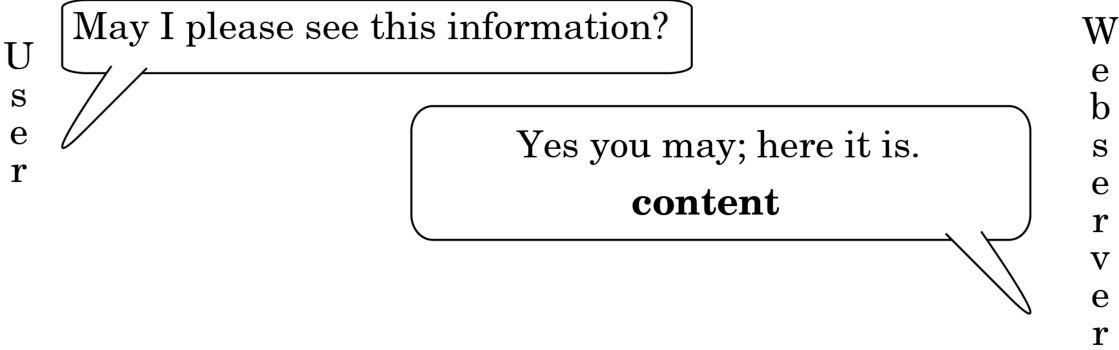
\includegraphics[width=0.8\textwidth]{diagrams/noauth2}
	  \caption{An HTTP request without authentication, as portrayed by humans.}
		\label{fig:humnoauth}
	\end{figure}
	
	\begin{figure}[ht!]
	  \centering
	  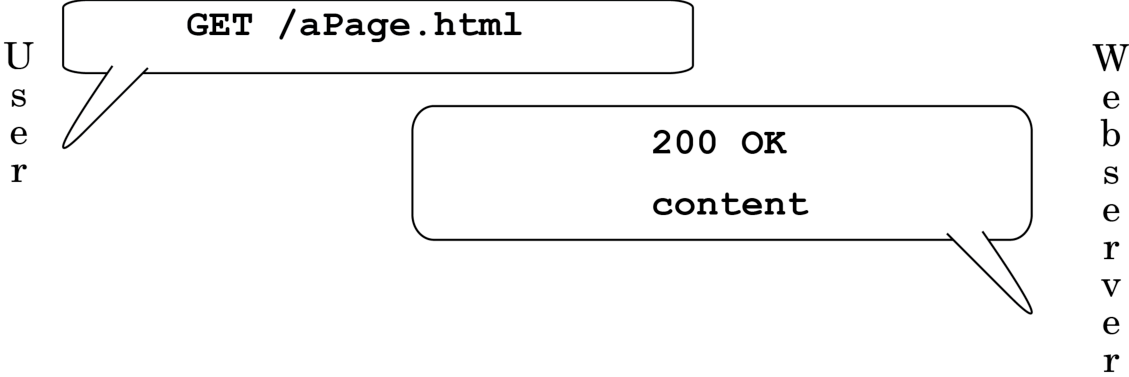
\includegraphics[width=0.8\textwidth]{diagrams/noauth2-2}
	  \caption{An HTTP request without authentication.}
		\label{fig:compnoauth}
	\end{figure}
		
	If the owner of a server wishes to restrict access to a particular document or set of documents, the owner can instruct the web server to do so. The librarian will ask the human for a proof of identity, and provide the document only if the identity is on the list, as in Figure~\ref{fig:humauthsuccess}. The server's HTTP request for identification is the code ``401 Not Authorized;'' this code tells the client device that some proof of identity is required. When the client receives the request, it will send an Authorization command, complete with username and password. (It may send the username and password in one of several encodings, but the command is otherwise the same.) The HTTP version of this request is shown in Figure~\ref{fig:compauthsuccess}. If the server recognizes the username and password, it will send 200 OK, along with the requested document---just as it did in Figure~\ref{fig:compnoauth}.
	
	\begin{figure}[ht!]
	  \centering
	  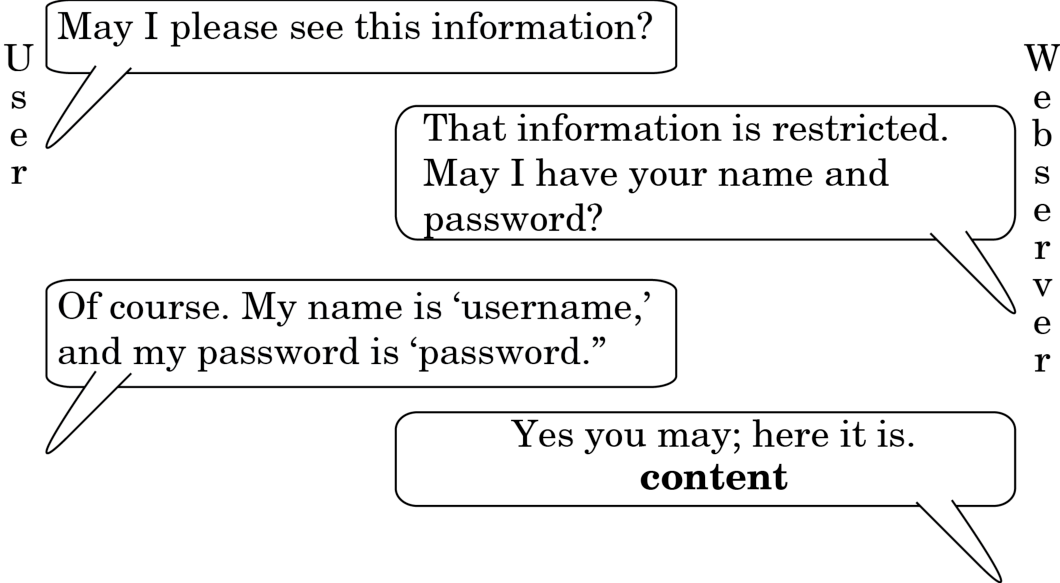
\includegraphics[width=0.8\textwidth]{diagrams/authsuccess2}
	  \caption{An HTTP request with successful authentication, as portrayed by humans.}
		\label{fig:humauthsuccess}
	\end{figure}
	
	\begin{figure}[ht!]
	  \centering
	  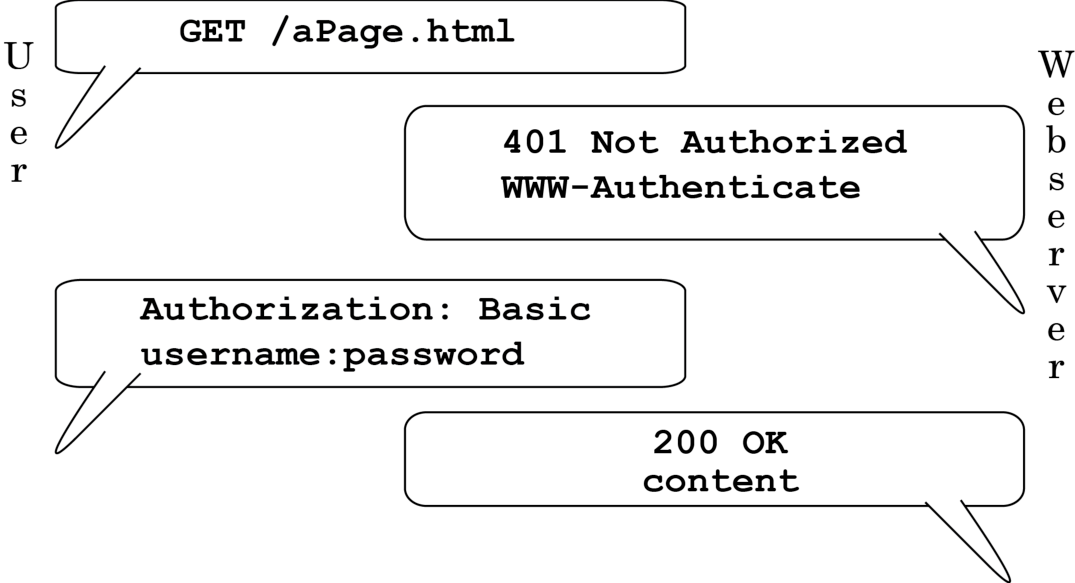
\includegraphics[width=0.8\textwidth]{diagrams/authsuccess2-2}
	  \caption{An HTTP request with successful authentication.}
		\label{fig:compauthsuccess}
	\end{figure}
	
	If our librarian does not accept the provided identification, he will refuse to provide the document, as shown in Figure~\ref{fig:humauthfail}. If the server does not recognize the username and password, it will send code: ``403 Forbidden.'' This indicates that the username and password is not known to the server, or is not authorized to access the particular document. This flow is shown in Figure~\ref{fig:compauthfail}; note that no content is sent by the server in that case.
	
	\begin{figure}[ht!]
	  \centering
	  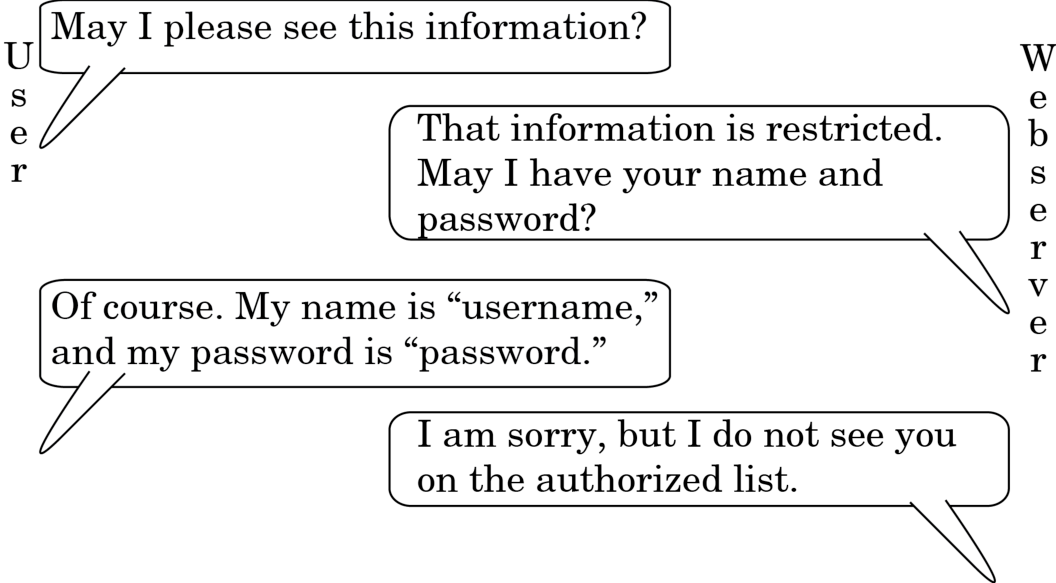
\includegraphics[width=0.8\textwidth]{diagrams/authfail2}
	  \caption{An HTTP request with unsuccessful authentication, as portrayed by humans.}
		\label{fig:humauthfail}
	\end{figure}
	
	\begin{figure}[ht!]
	  \centering
	  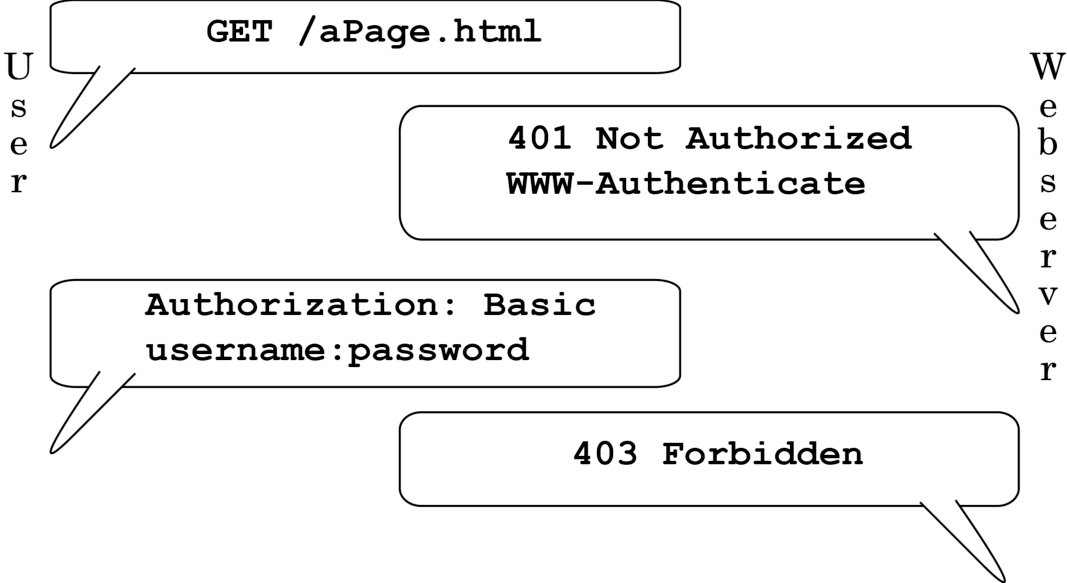
\includegraphics[width=0.8\textwidth]{diagrams/authfail2-2}
	  \caption{An HTTP request with unsuccessful authentication.}
		\label{fig:compauthfail}
	\end{figure}
	
	
	AT\&T instructed its servers that the email addresses it had were unrestricted content, available to anyone; in essence, they were the content for a particular set of documents. The documents were named for their associated numeric identifiers, called ICC-IDs.\footnote{A Subscriber Identity Module, or ``SIM Card,'' is a small replaceable chip inside mobile phones or other mobile devices that use the Global System for Mobile Communications (GSM) protocol; in the United States, AT\&T and T-Mobile use GSM. An Integrated Circuit Card Identifier, or ICC-ID, is a number up to twenty digits in length that identifies a SIM card. It is important to note that an ICC-ID is not an authenticating number; it could be compared to a football player's jersey number, in that it was not designed to be used for anything more than the most transient identification.} If our librarian is asked for several documents in a row, each by its identifier, there is no issue; it responds to each in turn. If it cannot find a document that corresponds to an identifier, it simply responds that while it has verified that the document number is valid, it has no information to give on that document.\footnote{This is because AT\&T's server would respond the same way to each request, regardless of whether it knew a particular ICC-ID; if it did not know an ID, it would simply fail to provide an email address in that otherwise-blank space. A server could also be configured to give the response ``404 Not Found,'' if it encountered an ID of which it had not heard.} This is shown in Figure~\ref{fig:humipad}.	Mr. Spitler simply requested many documents; for each, AT\&T's server returned a ``200 OK,'' with either the email address of a subscriber or a notice that it was not known, as shown in Figure~\ref{fig:compipad}.
	
	\begin{figure}[ht!]
	  \centering
	  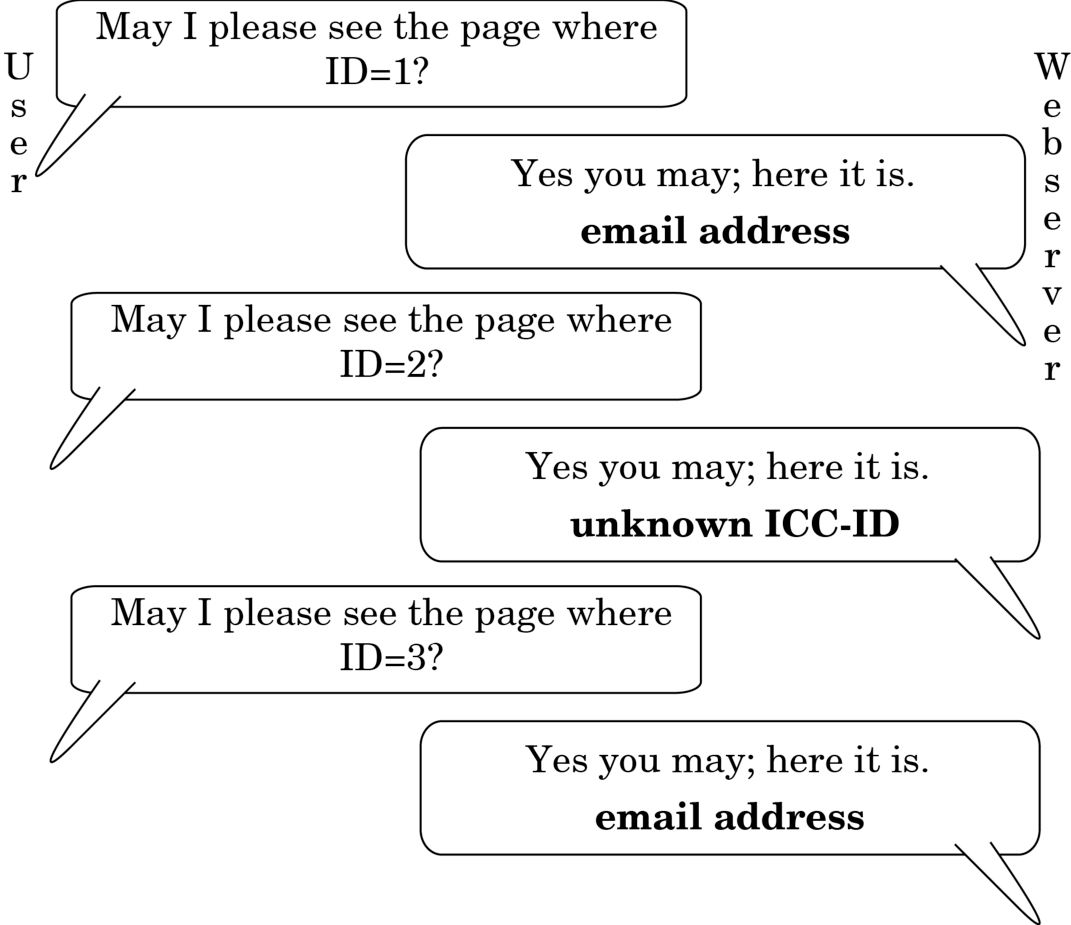
\includegraphics[width=0.8\textwidth]{diagrams/ipad2}
	  \caption{Mr. Spitler's requests to the AT\&T server, as portrayed by humans.}
		\label{fig:humipad}
	\end{figure}

	\begin{figure}[ht!]
	  \centering
	  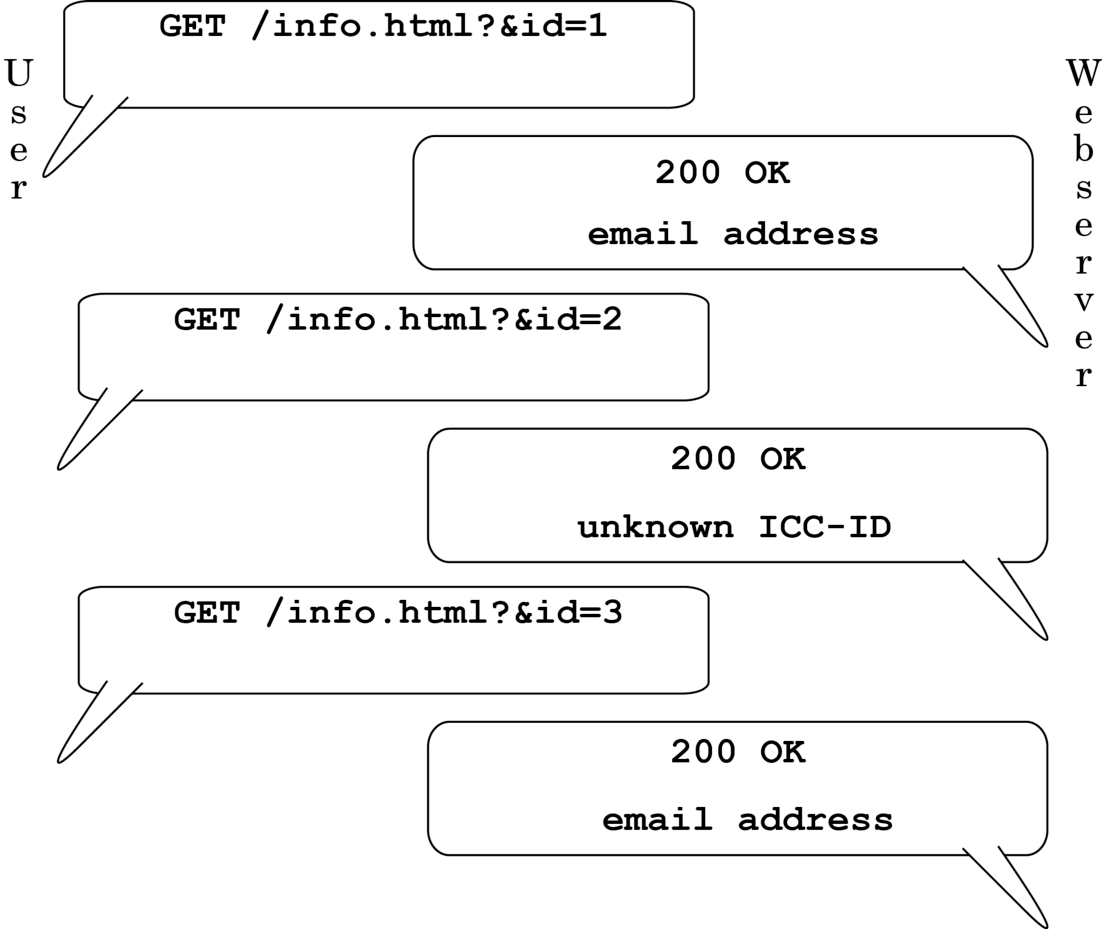
\includegraphics[width=0.8\textwidth]{diagrams/ipad2-2}
	  \caption{Mr. Spitler's requests to the AT\&T server.}
		\label{fig:compipad}
	\end{figure}
	
	It is crucial to realize that AT\&T gave the webserver its instructions: they \emph{explicitly} told it to respond with consumers' private information to anyone who gave the server a valid number, easily picked at random. With this action, AT\&T deliberately made the information public to anyone who asked, set no limits whatsoever on who could ask or how often, and required no verification before handing out ostensibly private information to all comers. AT\&T used technical means to signal to any user of the Internet that this data was public, not private, and treated the data accordingly.
	
	While the repeated requests outlined in Figure~\ref{fig:compipad} might look odd to a lay person, they in fact represent the standard operation of the Web. A user makes these same requests whenever they use a website, whether they are clicking through cat videos, using a search engine, or reading a blog. Indeed, if a person wished to read every post on a blog in order, they might first ask for \url{http://www.example.com/blog/1}, signifying the first post; having read that, they would ask for \url{http://www.example.com/blog/2}, the second post; \url{http://www.example.com/blog/3}, the third post; and so on. (This might be done through clicking on links, or it might be done by manually changing the address displayed to the user.) There is nothing untoward about this behavior; it is the default behavior for most of the Web, and these requests are set out and sent in the same way, regardless of what device sends them, or whether a user is present.
	
	\subsubsection{AT\&T's secret determination of ``authorized access'' creates an unconstitutional private law}
	
	It is a fundamental violation of the basic concept of due process for an act to be secretly criminal; AT\&T's determination that access to documents it had made public was unauthorized, without making such a determination public in any way, amounts to the creation of a private law. 
	
	\begin{quote}
		\begin{singlespace}
			\fontsize{14}{17}\selectfont
	``The rule that `ignorance of the law will not excuse' is deep in our law, as is the principle that of all the powers of local government, the police power is `one of the least limitable.' On the other hand, due process places some limits on its exercise. Engrained in our concept of due process is the requirement of notice.'' \emph{Lambert v. People of the State of California}, 355 U.S. 225, 228, 78 S.Ct. 240 (1957) (citations omitted).\index[case]{\emph{Lambert v. People of the State of California}, 355 U.S. 225, 78 S.Ct. 240 (1957)}
		\end{singlespace}
	\end{quote}
	
	 In \emph{Lambert}, the Supreme Court set out a theory of actual notice of a law. In the case at hand, however, Mr. Auernheimer had not even the \emph{possibility} of notice of the law in question; in effect, AT\&T's determination was secret, making it impossible for any legal scholar---let alone, any reasonable user of the Internet---to have knowledge of the legality of the action beforehand. AT\&T did not use any means at its disposal, whether through the display of a warning, or through utilizing the fundamental protocol of the World Wide Web's authorization mechanism, as described in Section~\ref{subsubsec:www}, to give notice that access of the type Mr. Auernheimer aided was unauthorized. In fact, AT\&T declared, at the time that the documents were accessed, that the access was authorized; instead of using the ``403 Forbidden'' code to signify a lack of authorization, as shown in Figure~\ref{fig:compauthfail}, it instead used the ``200 OK'' code that signifies that no further authorization is needed, as shown in Figure~\ref{fig:compnoauth}. This means that Mr. Auernheimer cannot be held legally responsible for exceeding his ``authorized access,'' since he had no way of finding out what access was ``unauthorized,'' and was indeed told by AT\&T's computers that his access was authorized.
	 
	 Moreover, to affirm the district court would provide for the enforcement of such private laws, and the handling of litigation about them, at public expense.  The criminal justice system is ill-suited to serve as a tool for corporate policy interests.  If a business fails to take care to avoid unwanted consequences associated with its publication of information, it cannot later be allowed to convert those consequences into felonies for the criminal justice system to handle; to permit that path would allow businesses to shirk their duty to safeguard private information, and simply pass the workload onto an on already overburdened court system.
		
	The Ninth Circuit has already rejected a system of private laws, even \emph{with} notice, being used to turn a user's access to data into a felonious act under the CFAA. In \emph{U.S. v. Nosal}, 676 F.3d 854 (9th Cir. 2012),\index[case]{\emph{U.S. v. Nosal}, 676 F.3d 854 (9th Cir. 2012)} the Ninth Circuit ruled that it would not allow ``every violation of a private computer use policy [to be] a federal crime.'' \emph{Id.} at 859.\index[case]{\emph{U.S. v. Nosal}, 676 F.3d 854 (9th Cir. 2012)} 
	\begin{quote}
		\begin{singlespace}
			\fontsize{14}{17}\selectfont
			``[T]he government's proposed interpretation of the CFAA allows private parties to manipulate their computer-use and personnel policies so as to turn these relationships into ones policed by the criminal law.'' \emph{Id.} at 860.\index[case]{\emph{U.S. v. Nosal}, 676 F.3d 854 (9th Cir. 2012)}
		\end{singlespace}
	\end{quote}
		
		 We invite this Court to adopt the Ninth Circuit's determination that this sort of private legal scheme is unacceptable in a society of laws.
	
	\subsubsection{AT\&T's post-hoc determination of ``authorized access'' violates the Ex Post Facto Clause}
	
	The Computer Fraud and Abuse Act criminalizes the act of exceeding authorized access to a computer, and defines authorization solely as what the user is ``entitled'' to access. 18 U.S.C. \S1030(e)(6).\index[statute]{10 U.S.C. \S1030} As explained in Section~\ref{subsubsec:www}, AT\&T used technical means to make public the private information of its customers, as a response to anyone who asked for it; a reasonable user of the World Wide Web would assume that data explicitly made public would be public. However, after the data was accessed, AT\&T decided that this information that it had made public should, in retrospect, have been private, and thus no user should have access to it (despite the fact that it was being handed out by their server, at their behest). This determination, insofar as it is adopted by the United States, and used as the threshold for criminal liability, makes an action criminal that was non-criminal when it was taken; as such, it amounts to a violation of the Ex Post Facto Clause of the United States Constitution.
	
	Ex post facto laws are prohibited by Article 1, Section 9 of the United States Constitution; this means that something cannot be made illegal, and a person thereby be held liable, for an action taken before the illegality had been designated. Ex post facto laws have been broadly defined:
	
	\begin{quote}
		\begin{singlespace}
			\fontsize{14}{17}\selectfont
		``1st. Every law that makes an action done before the passing of the law, and which was innocent when done, criminal; and punishes such action. 2d. Every law that aggravates a crime, or makes it greater than it was, when committed. 3d. Every law that changes the punishment, and inflicts a greater punishment, than the law annexed to the crime, when committed. 4th. Every law that alters the legal rules of evidence, and receives less, or different, testimony, than the law required at the time of the commission of the offence, in order to convict the offender.''  \emph{Calder v. Bull}, 3 Dall. 386, 390, 1 L.Ed. 648 (1798) (emphasis deleted).\index[case]{\emph{Calder v. Bull}, 3 Dall. 386, 1 L.Ed. 648 (1798)}
		\end{singlespace}
	\end{quote}
	
	Particularly relevant here, an ex post facto law need not be a complete legislative action for it to violate the Ex Post Facto Clause (i.e., it need not be an actual law). Instead, it need only have ``binding legal effect,'' as the Supreme Court restated in \emph{Peugh v. U.S.}, 569 U.S. \_\_\_, at *12, 133 S.Ct. 2072 (2013).\index[case]{\emph{Peugh v. U.S.}, 569 U.S. \_\_\_, 133 S.Ct. 2072 (2013)} 
	
	In \emph{Peugh}, the Supreme Court held that even non-binding sentencing guidelines---guidelines that did not carry the force of law, and were not created through direct Congressional action---could violate the Ex Post Facto Clause. Here, the imposition of liability is actually more concerning than the stricken sentence in \emph{Peugh}: AT\&T, a non-governmental, non-neutral corporation, created the rule Mr. Auernheimer is charged with violating, after the time at which it is claimed that he violated it. While \emph{Peugh} dealt with sentencing guidelines, the \emph{amici} believe that the rule put forward need not be restricted to strictly governmental action; this non-governmental action created the requisite ``binding legal effect,'' and, crucially, the determination was subsequently adopted by the government when it chose to indict Mr. Auernheimer. In this case, AT\&T made an after-the-fact determination that an action, already taken, had violated some previously-unarticulated rule; this determination meant that an action that in other respects was simply a request to view a web page, as explained in Section~\ref{subsubsec:www}, was now criminal. This determination, and its subsequent adoption by the United States, has had the requisite ``binding legal effect'' upon Mr. Auernheimer in the form of the case at bar.
	
	In \emph{Peugh}, the Supreme Court held that even intervening discretionary acts could not save a sentencing guideline: ``[O]ur cases make clear that `[t]he presence of discretion does not displace the protections of the Ex Post Facto Clause.'\,'' \emph{Peugh}, 569 U.S. at *12 (citation omitted).\index[case]{\emph{Peugh v. U.S.}, 569 U.S. \_\_\_, 133 S.Ct. 2072 (2013)} In this case, AT\&T issued much more than a mere guideline---it, through the government's adoption of its determination, issued the new rule of law itself, after the act had been committed. \emph{Peugh} holds that no discretion between then and now, such as the issuance of an indictment, prevents the situation from violating the Ex Post Facto Clause. As such, Mr. Auernheimer may not be held criminally liable for violating a law not fully actualized until after his act.
	
	\subsection{Criminalizing access to publicly-offered material is not in the public interest, because it prevents the security research community from exercising its consumer-protecting role.}
	
	Mr. Auernheimer is one example of a security researcher, a profession of which the amici are also a part. There are many thousands of security researchers worldwide\footnote{One security research conference, the annual DEF CON conference in Las Vegas, NV, had more than 13,000 attendees in 2012.} who work in government, academia, and for private industry. They have a shared goal: to protect people from dangerous computer systems, whether they be websites that leak personal information, implantable cardioverter-defibrillators that are susceptible to remote disabling, or dams that can be controlled---or even destroyed---from anywhere in the world.\footnote{Talks on each of these were presented at DEF CON in 2012, among many other presentations.} The security research community is a part of the larger consumer safety community: as with more traditional product safety researchers, security researchers form an important part of the system of consumer protection.
	
	The role that consumer safety and advocacy organizations and researchers play in ensuring the safety of the population has been recognized throughout the legal system. \emph{See, e.g.,} 
	The Consumer Product Safety Act, 15 U.S.C. \S2051, \emph{et seq.} (2006) (providing protection for those who ``blow the whistle'' on violations of consumer safety),\index[statute]{15 U.S.C. \S2051}
	\emph{National Ass'n Of State Utility Consumer Advocates v. F.C.C.}, 457 F.3d 1238 (11th Cir. 2006) (cellular telephone service billing irregularities),\index[case]{\emph{National Ass'n Of State Utility Consumer Advocates v. F.C.C.}, 457 F.3d 1238 (11th Cir. 2006)}
	\emph{International Healthcare Management v. Hawaii Coalition For Health}, 332 F.3d 600 (9th Cir. 2003) (medical care pricing),\index[case]{\emph{International Healthcare Management v. Hawaii Coalition For Health}, 332 F.3d 600 (9th Cir. 2003)}
	\emph{Kaiser Aluminum \& Chemical Corp. v. U. S. Consumer Product Safety Commission}, 574 F.2d 178 (3d Cir. 1978) (aluminum house wiring),\index[case]{\emph{Kaiser Aluminum \& Chemical Corp. v. U. S. Consumer Product Safety Commission}, 574 F.2d 178 (3d Cir. 1978)}
	\emph{Grimshaw v. Ford Motor Co.}, 191 CA3d 757, 236 Cal. Rptr. 509 (Cal. Ct. App. 1981) (the Ford Pinto case),\index[case]{\emph{Grimshaw v. Ford Motor Co.}, 191 CA3d 757, 236 Cal. Rptr. 509 (Cal. Ct. App. 1981)}
	    \emph{In re Harvard Pilgrim Health Care, Inc.}, 434 Mass. 51, 746 N.E.2d 513 (Mass. 2001) (medical care organizations),\index[case]{\emph{In re Harvard Pilgrim Health Care, Inc.}, 434 Mass. 51, 746 N.E.2d 513 (Mass. 2001)}
			 \emph{Porter v. South Carolina Public Service Com'n}, 333 S.C. 12, 507 S.E.2d 328 (S.C. 1998) (BellSouth statewide rate-setting corruption),\index[case]{\emph{Porter v. South Carolina Public Service Com'n}, 333 S.C. 12, 507 S.E.2d 328 (S.C. 1998)}
		 \emph{Utah State Coalition of Sr. Citizens v. Utah Power and Light Co.}, 776 P.2d 632 (Utah 1989) (protecting the elderly from a state power monopoly).\index[case]{\emph{Utah State Coalition of Sr. Citizens v. Utah Power and Light Co.}, 776 P.2d 632 (Utah 1989)} These organizations do not ask for, nor do they require, the permission of the companies whose publicly-accessible products they test for problems that endanger the safety of society at large, and every member of society specifically. If there were such a requirement, the permission would in reality never be given; as in the case at hand, the existence of the problem in the first place, combined with either a lack of awareness on the part of the responsible company, or the company's unwillingness to fix the problem, would be embarassing to the company.
	
	There are relatively few sources of pressure to fix design defects, whether they be in wiring, websites, or cars. The government is not set up to test every possible product or website for defects before its release, nor should it be; in addition, those defects in electronic systems that might be uncovered by the government (for instance, during an unrelated investigation) are often not released, due to internal policies. Findings by industry groups are often kept quiet, under the assumption that such defects will never come to light---just as in \emph{Grimshaw} (the Ford Pinto case).\index[case]{\emph{Grimshaw v. Ford Motor Co.}, 191 CA3d 757, 236 Cal. Rptr. 509 (Cal. Ct. App. 1981)} The part of society that consistently serves the public interest by finding and publicizing defects that will harm consumers is the external consumer safety research community, whether those defects be in consumer products or consumer websites. In the situation at hand, AT\&T was improperly safeguarding the personal information of hundreds of thousands of consumers. When Mr. Auernheimer discovered this fact, he publicized it, in precisely the same way that Consumers Union, publisher of \emph{Consumer Reports}, does with each consumer-safety violation that it uncovers: he made it available to the press.
		
	The United States would like this Court to create a rule that would allow private corporations to control the right of researchers to examine public accommodations, as long as those accommodations were on the Internet. If that rule were applied to the physical world, it would be unlawful for a worker to report a building code violation on a construction site. It would be unlawful for an environmental activist to sample water for contaminants, lest they come across things a company (which had illegally dumped waste in a river) deemed secret. It would be unlawful for a customer at a restaurant to report a rat running across his or her table to the city health authority. It would be unlawful for a newspaper to investigate whether a business is illegally discriminating against racial minorities. It would even be illegal for Ralph Nader to have published (or have done the research for) ``Unsafe at Any Speed;'' his analysis of design flaws inherent to certain automobiles, found while examining the design of those automobiles without permission from their manufacturers, would be illegal under a system that required that a company give its consent to any research of which it might not approve. 
	
	In fact, every car sold today contains a great deal of computers that control every facet of the car's operation---from entertainment systems, to how the engine runs, and even braking. The CFAA interpretation proposed by the government could be used to criminalize Mr. Nader's research; if such research were done today, analysis of the car would necessarily involve its computers. General Motors should not have been allowed, after the fact, to decide that it had not meant to allow Mr. Nader access to the Chevrolet Corvair when Mr. Nader, rather than simply driving the car (with its inherent risks) as they had intended, instead used the car to discover its design risks and flaws and to make that information available to the public.	In short, private corporations would, under the rule proposed by the United States, be able to silence critics with the threat of imprisonment for publishing unfavorable research.
	
	In addition, the government, private corporations, and indeed the whole world have benefited from the research being done by independent security researchers. One flaw, discovered by one of the \emph{amici}, Dan Kaminsky, affected the core naming infrastructure of the Internet; his publication of the vulnerability to the affected entities---private corporations, governments, and open source projects---resulted in the aversion of a catastrophe; in essence, the flaw would have meant the complete destruction of the Internet. Members of the \emph{amici} have reported vulnerabilities in software created by Microsoft, VeriSign, McAfee, and many others of the world's largest corporations, whose software is used by millions of people every day. These researchers have prevented untold financial and privacy losses to entities large and small; it is therefore crucial that their continued right to research be protected.
	
	There is no reason why the electronic world and the physical world should differ so mightily: as an increasing amount of an average person's day-to-day life moves online (from paying bills to registering cars, and from shopping, to trading stocks, to musical performance and art appreciation), any conceivable rationale for this difference becomes facially unconvincing. The increased prominence of the digital world means that more scrutiny, not less, should apply to those who offer up public accommodations on the Internet (or in any digital forum). If, as Justice Brandeis once said, sunlight is to be a disinfectant, then it is imperative that if a public corporation chooses to endanger the safety of consumer information, we allow security researchers to publish their results and warn the public at large.
	
	\section{Conclusion}
	
	The United States asks this Court to endorse the use of the criminal justice system to cover up a private corporation's failures. AT\&T published private consumer data in an inappropriate fashion. Rather than take responsibility for their act, they have asked the criminal justice system to punish the researcher who uncovered their mistake. If this tactic is allowed to flourish, it will allow corporations to choose to terminate any safety oversight of their actions, and instead rely on the criminal process to serve as a cover-up for bad acts. Corporations will have no incentive to treat consumer data with adequate care in the future, since no one but the corporations themselves will be aware of any possible danger. In essence, the precedent that the respondent seeks to create is one that will make the American taxpayer subsidize the irresponsibility and misfeasance of private corporations through the courts on a scale never before seen.
	
	With this case, this Court has an opportunity to state that it is not acceptable for private corporations to warp the criminal justice system to shield themselves from public scrutiny in their digital public accommodations, any more than it is acceptable in any physical accommodation. Mr. Auernheimer's ``crime'' was to discover that a public corporation was giving anyone access to private consumer information; he discovered this by, in essence, repeatedly adding 1 to a number. The Court should not condone the metaphorical shooting of a messenger who acted for the safety and security of all. We ask that this Court overturn Mr. Auernheimer's conviction.
	
	\vspace{0.3in}
	
	\noindent Respectfully submitted,
	
	\vspace{0.2in}
	
	%Remove one of the next two lines to make either a signature line or a /s/ signature.
	
	%\vspace{0.3in}
	\noindent/s/ Alexander Muentz\\
	\noindent \line(1,0){200}	\\
	Alexander Charles Muentz \\
	Attorney for Amici
    
	\newpage
	
	\section{Certificate of Bar Membership}
	
	I, Alexander Charles Muentz, certify that I am a member in good standing of the Bar of the State of Pennsylvania, with Attorney ID 204459. I certify further that I am admitted to practice in the United States Court of Appeals for the Third Circuit.
	
	\section{Certificate of Compliance With Word Count Requirements}
	
	This brief complies with the type-volume limitation of Fed. R. App. P. 32(a)(7)(B)\index[statute]{28 U.S.C. Fed. R. App. P. 32}  and Fed. R. App. P. 29(d)\index[statute]{28 U.S.C. Fed. R. App. P. 29} because this brief contains 4,983 words, excluding the parts of the brief exempted by Fed. R. App. P. 32(a)(7)(B)(iii).\index[statute]{28 U.S.C. Fed. R. App. P. 32} This brief complies with the typeface requirements of Fed. R. App. P. 32(a)(5)\index[statute]{28 U.S.C. Fed. R. App. P. 32} and the type style requirements of Fed. R. App. P. 32(a)(6)\index[statute]{28 U.S.C. Fed. R. App. P. 32} because this brief has been prepared in a proportionally spaced typeface using TeX 3.1415926 in 14-Point New Century Schoolbook.
	
	\section{Certificate of Service}
	
	This brief was submitted through the CM/ECF system of the Third Circuit Court of Appeals; notice of its filing has been made through that system's Notice of Docket Activity.
	
	\section{Certificate of Identical Compliance of Briefs}
	
	The text of this brief is identical as submitted both in electronic format and in hard copy.
	
	\section{Certificate of Virus Check}
	
	This brief has been checked for malicious software by Wepawet, in the version made available on June 15, 2013.
	
\newpage

	\singlespace
	\fontsize{14}{17}
	\selectfont
	\thispagestyle{empty} % Gets rid of page number on the title page
	\begin{center}
		
		No. 13-1816
		
		\linethickness{0.5mm}
		\line(1,0){450}
		\vspace{-0.9em}
		\linethickness{0.25mm}
		\line(1,0){450}
		\vspace{0.20in}
		
		\textsc{In the United States Court of Appeals for the Third Circuit}
		\vspace{0.20in}
		
		\line(1,0){150}
		
		\vspace{0.20in}
		\textsc{United States of America,}
		\vspace{0.20in}
		\emph{Plaintiff-Appellee,}
		\vspace{0.05in}
		
		v.
		
		\vspace{0.20in}
		\textsc{Andrew Auernheimer,}
		\vspace{0.20in}
		\emph{Defendant-Appellant.}
		
		\line(1,0){150}
		
		\vspace{0.20in}
		Appeals from the United States District Court for the District of New Jersey, Case No. 11-CR-470, Judge Susan D. Wigenton
		\vspace{0.20in}
		
		\line(1,0){150}
		
		\vspace{0.20in}
		\textsc{Appendix of Meredith Patterson, Brendan O'Connor, Sergey Bratus, Gabriella Coleman, Peyton Engel, Matthew Green, Dan Hirsch, Dan Kaminsky, Samuel Liles, Shane MacDougall, Brian Martin, C.\ Thomas, and Peiter Zatko as Amici Curiae Supporting Appellant}
		\vspace{0.20in}
		
		\line(1,0){150}
		
		\vspace{0.20in}
		\textsc{Alex Muentz} \\
		Adjunct Instructor \\
		Department of Criminal Justice \\
		Gladfelter Hall, 5th floor \\
		Temple University \\ 
		1115 Polett Walk \\
		Philadelphia PA 19122 \\
		(215) 806-4383 \\
		\vspace{0.20in}

		
		\line(1,0){450}
		\vspace{-0.9em}
		\linethickness{0.5mm}
		\line(1,0){450}		
		\linethickness{0.25mm} %Just so if we want a normal line later, we'll have it
		
	\end{center}


	\newpage
	\setcounter{page}{1}
	\includepdfset{pages=-,pagecommand=\thispagestyle{fancy}}
	\fancyfoot[C]{\fontsize{14}{17}\selectfont App. \thepage}
	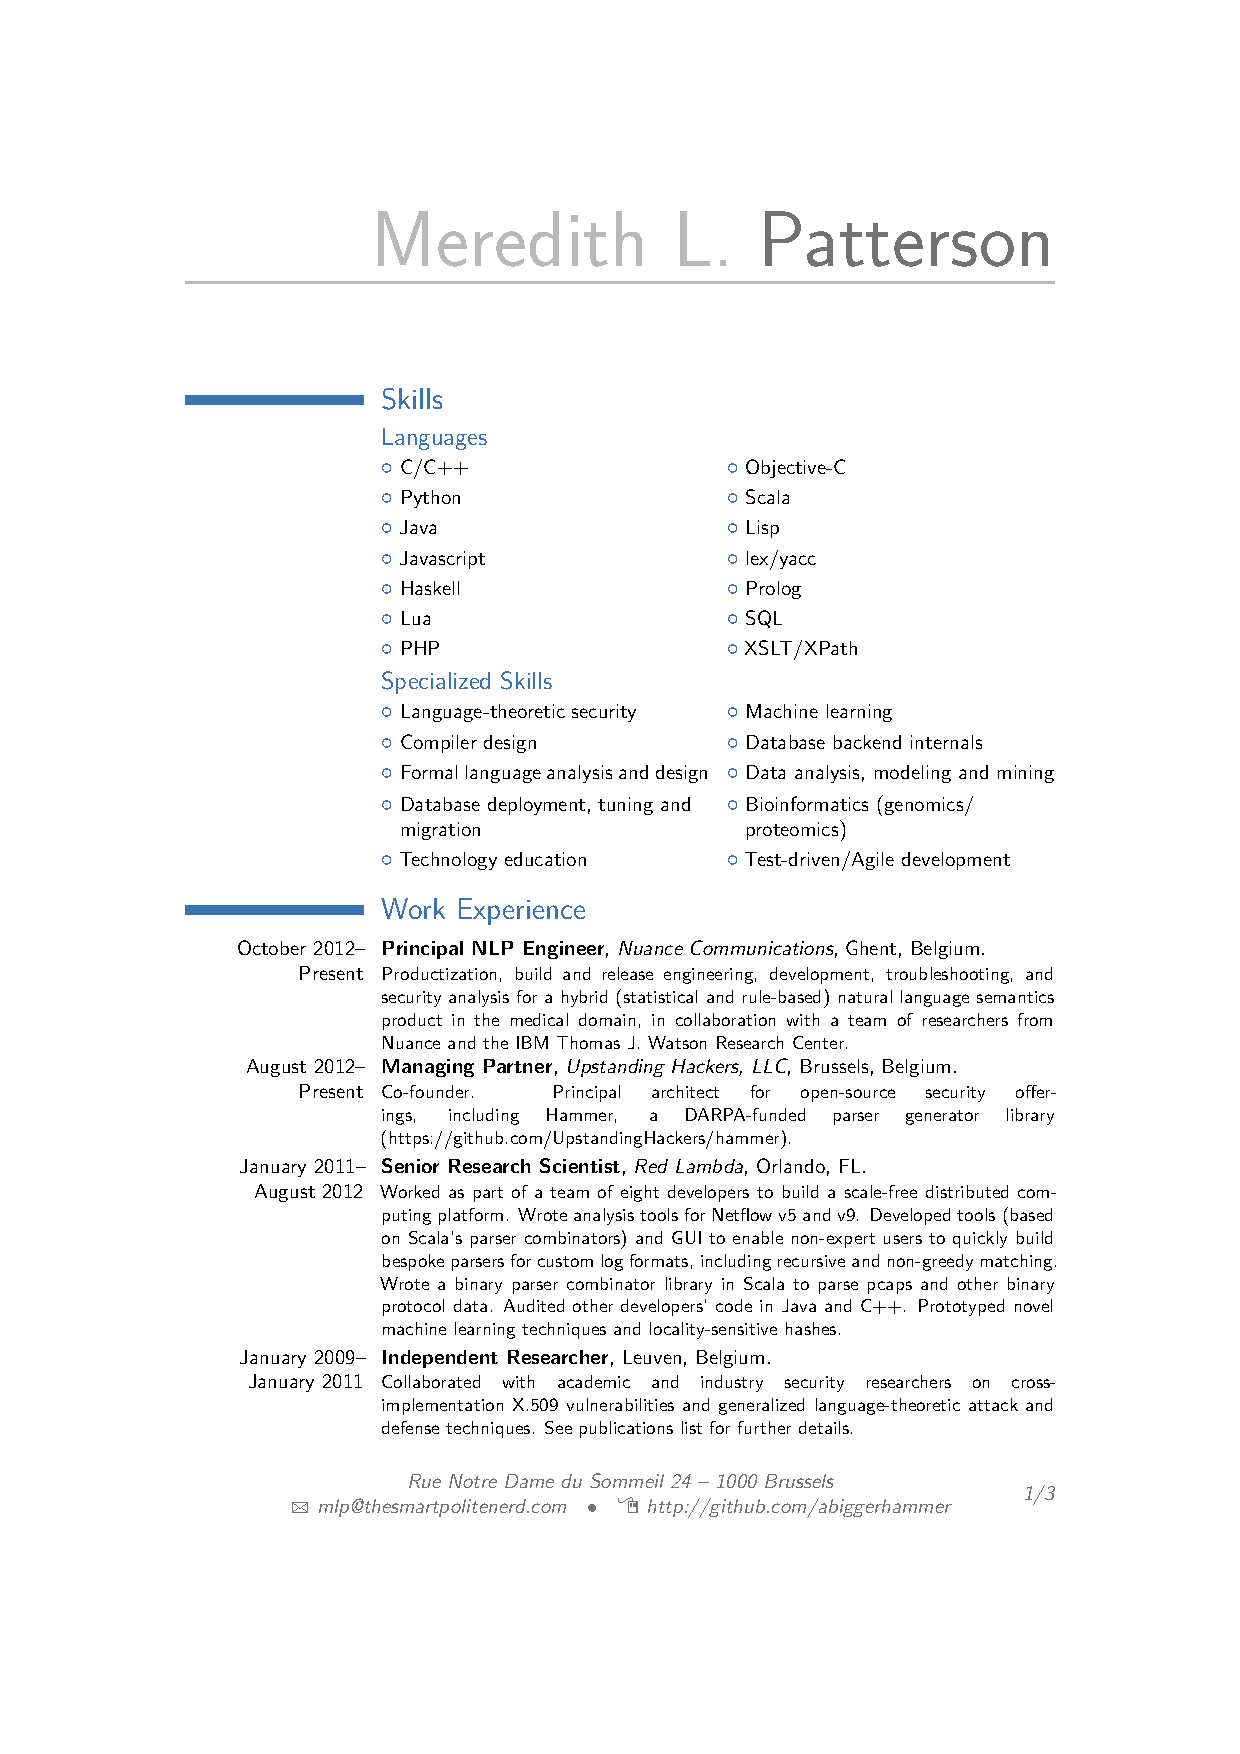
\includepdf[pages=-]{resumes/Patterson.pdf}
	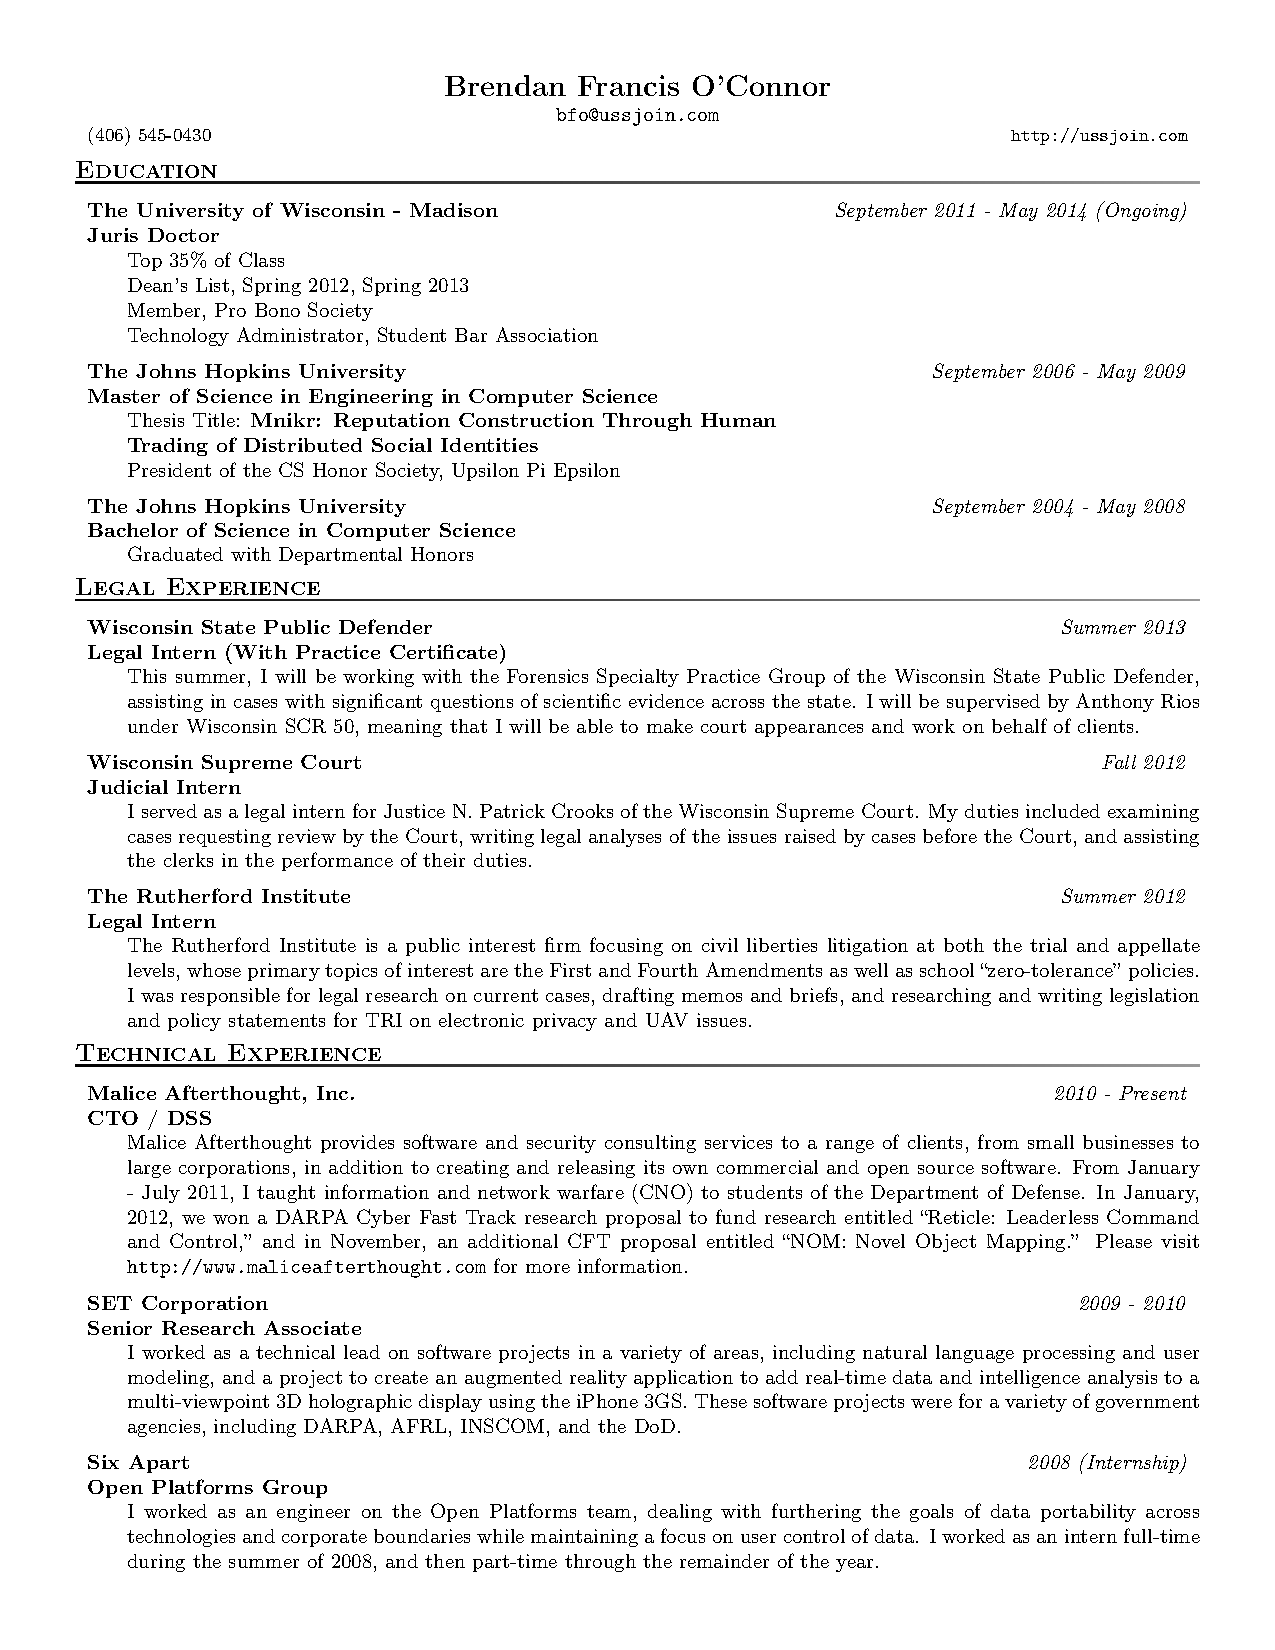
\includepdf[pages=-]{resumes/OConnor.pdf}
	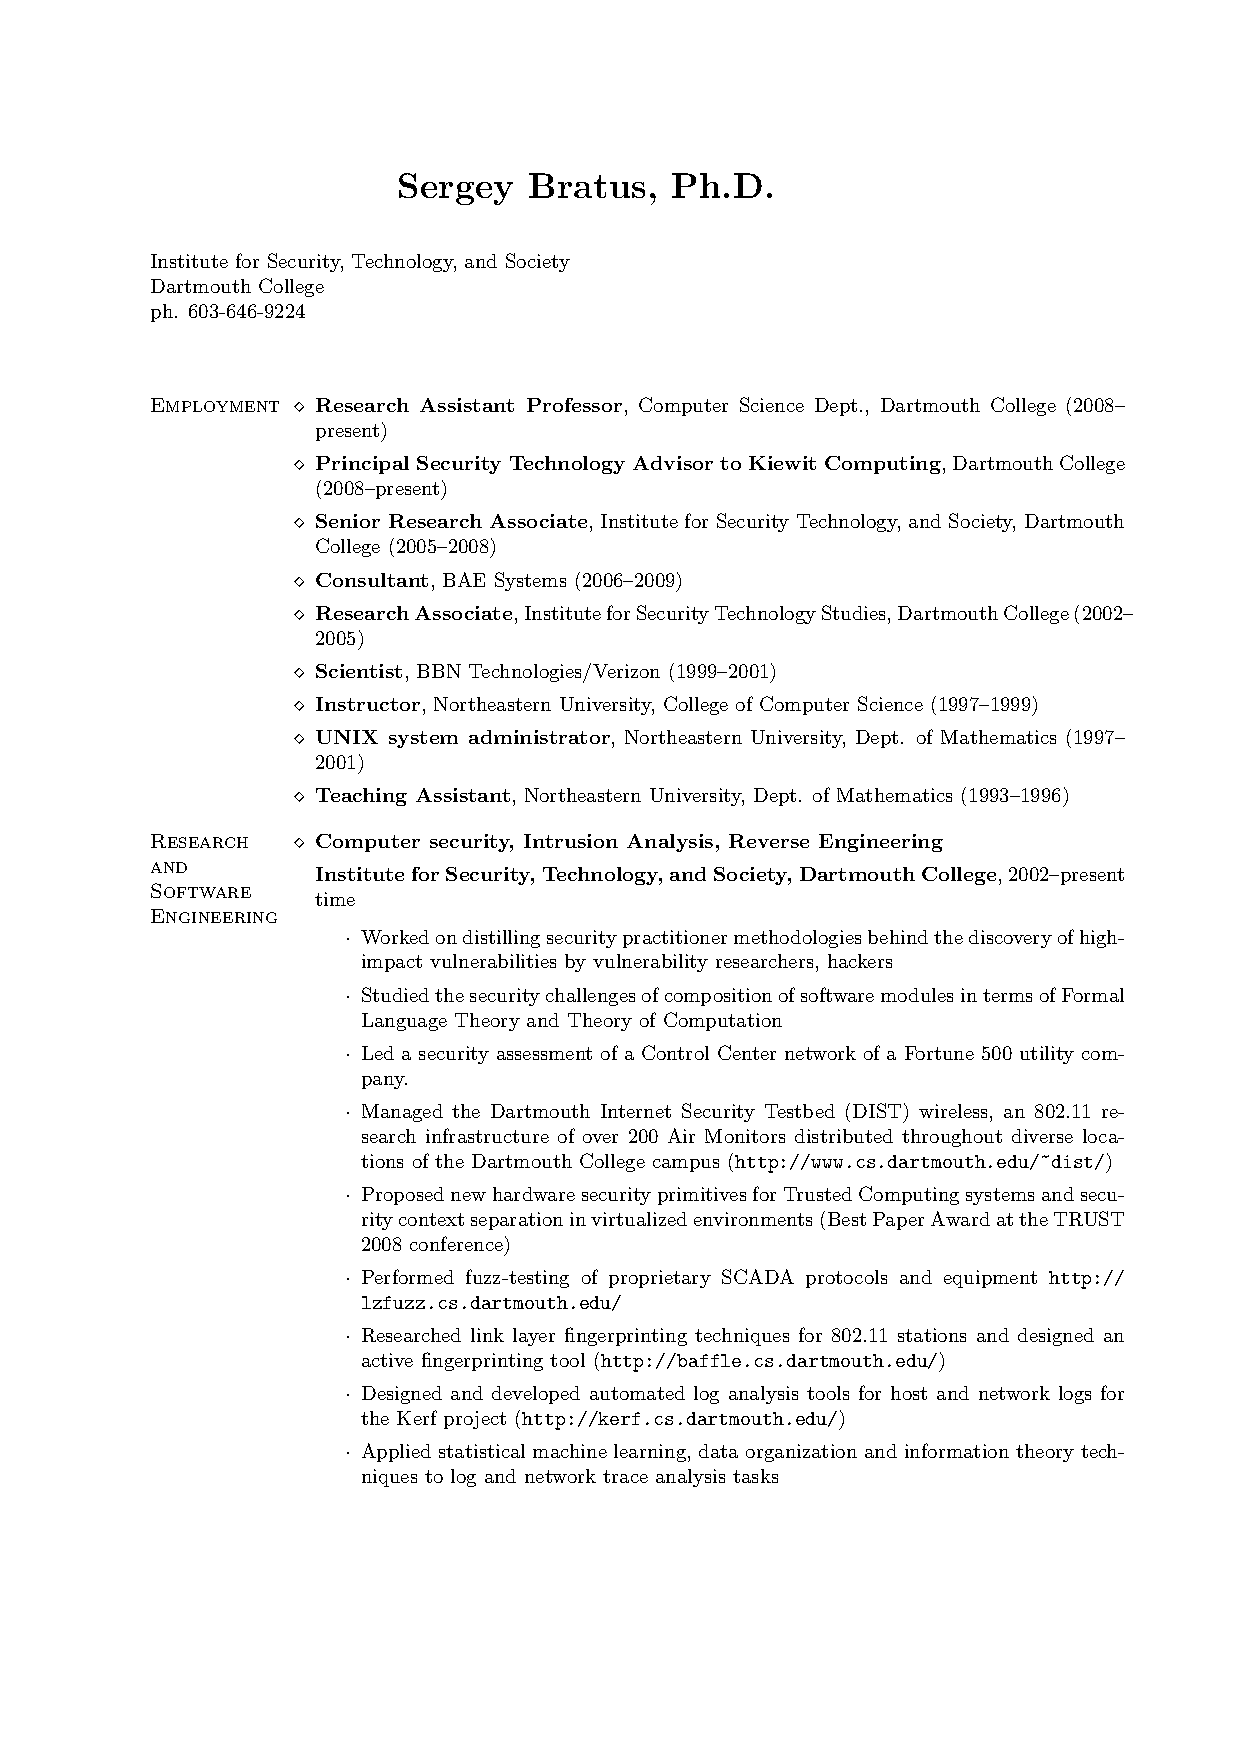
\includepdf[pages=-]{resumes/Bratus.pdf}
	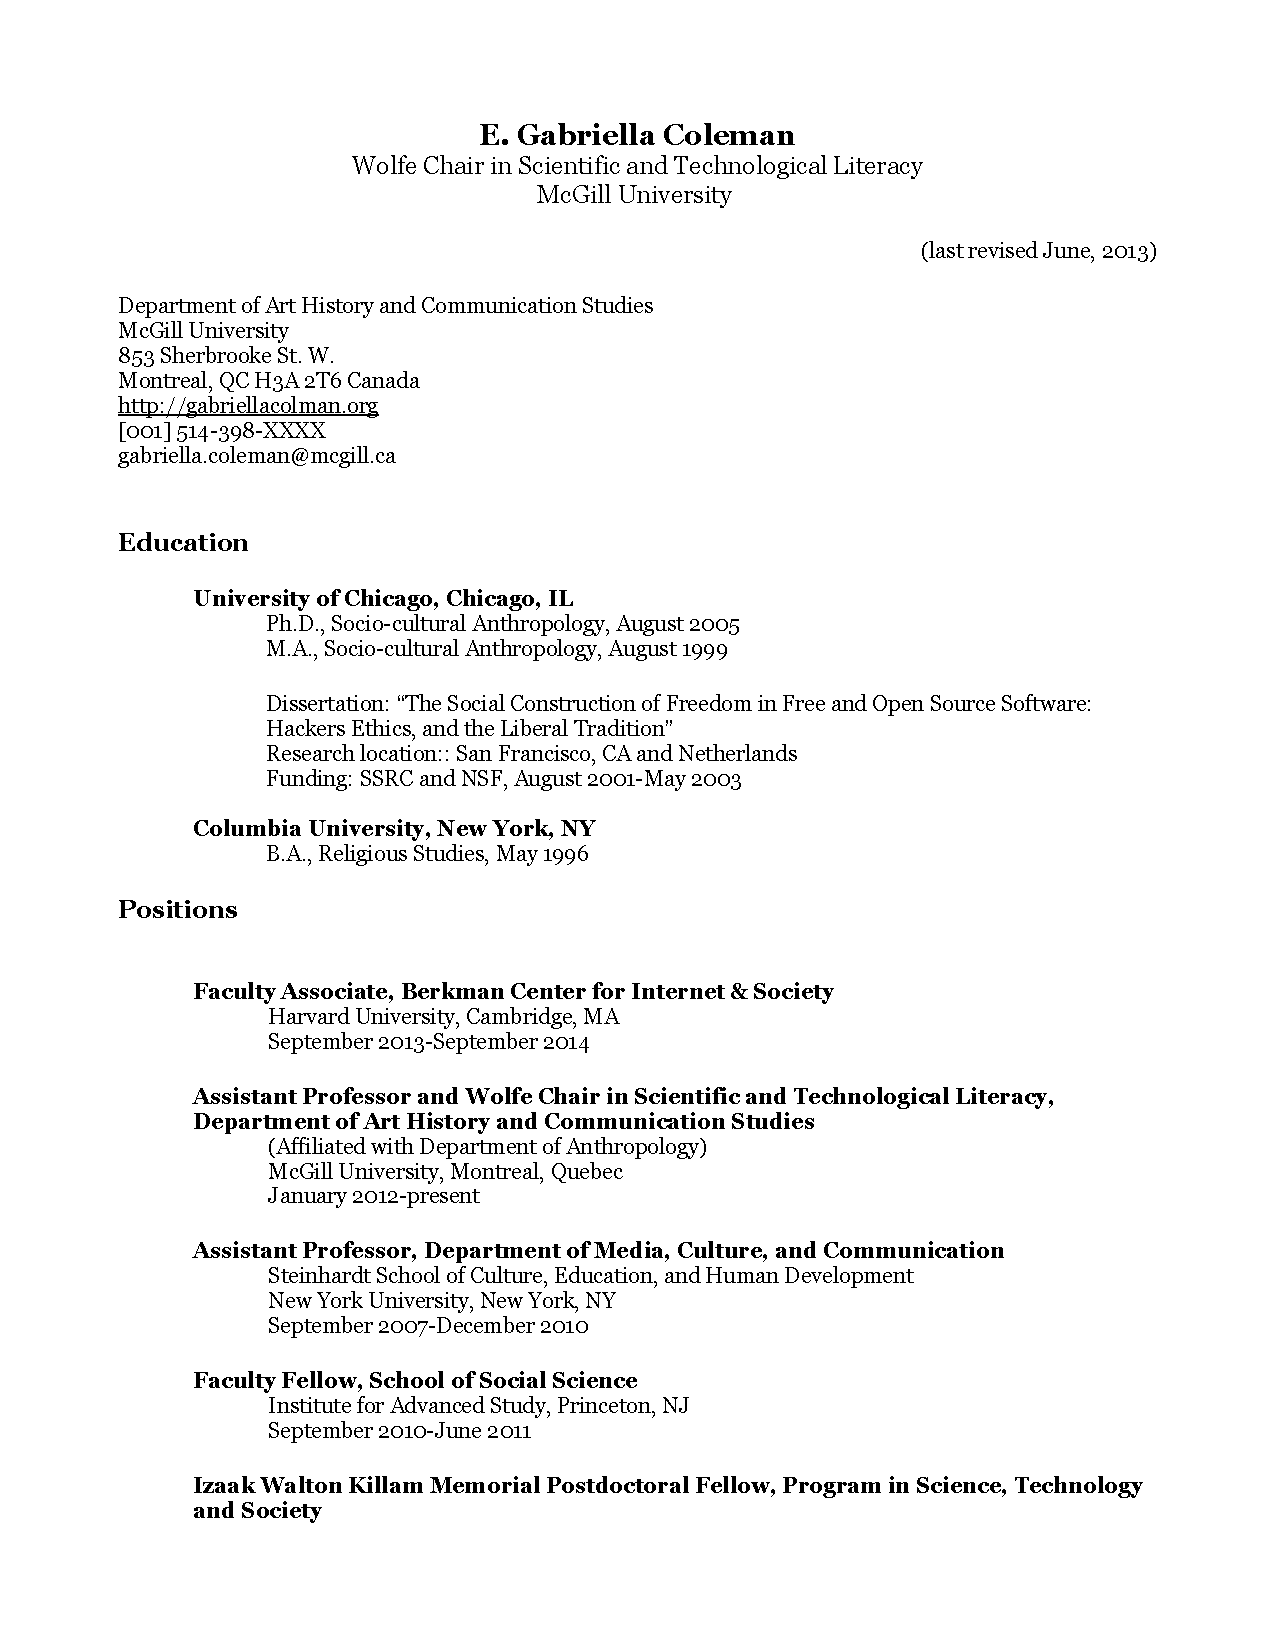
\includepdf[pages=-]{resumes/Coleman.pdf}
	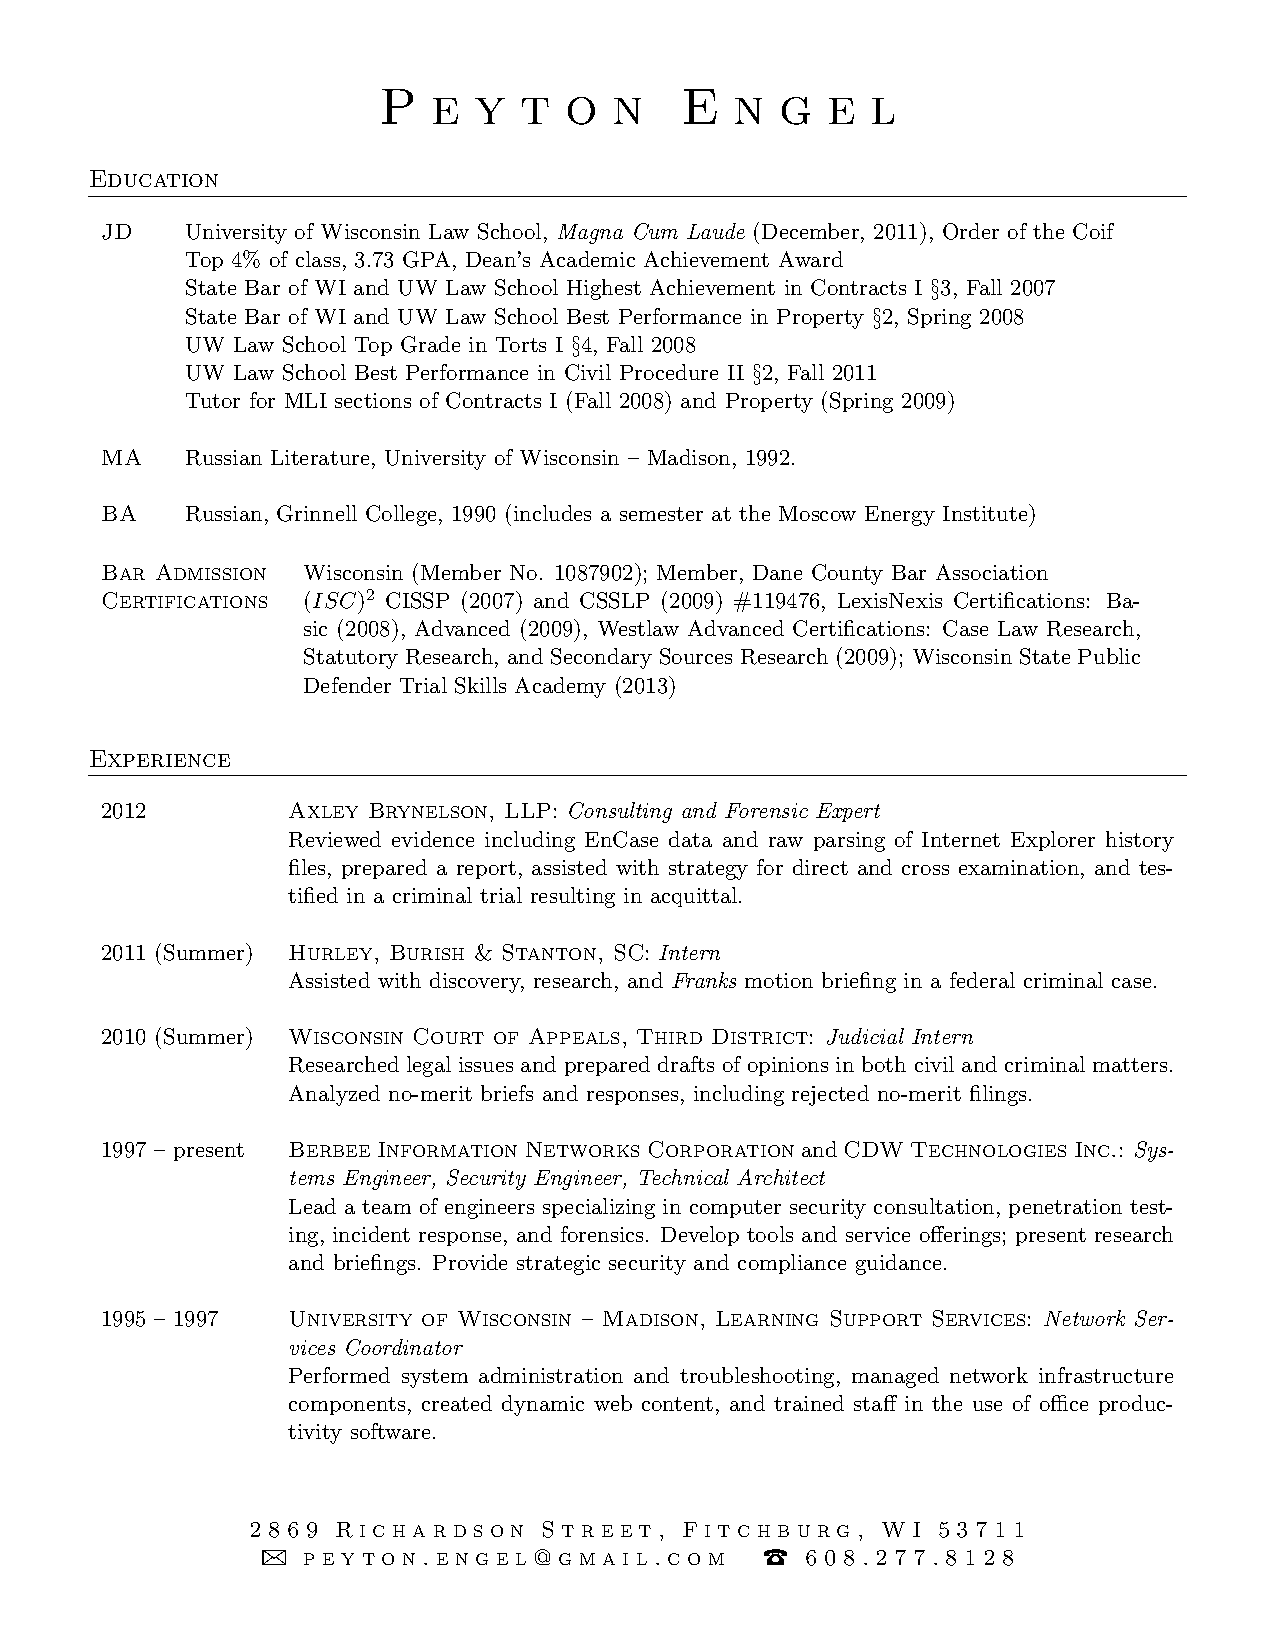
\includepdf[pages=-]{resumes/Engel.pdf}
	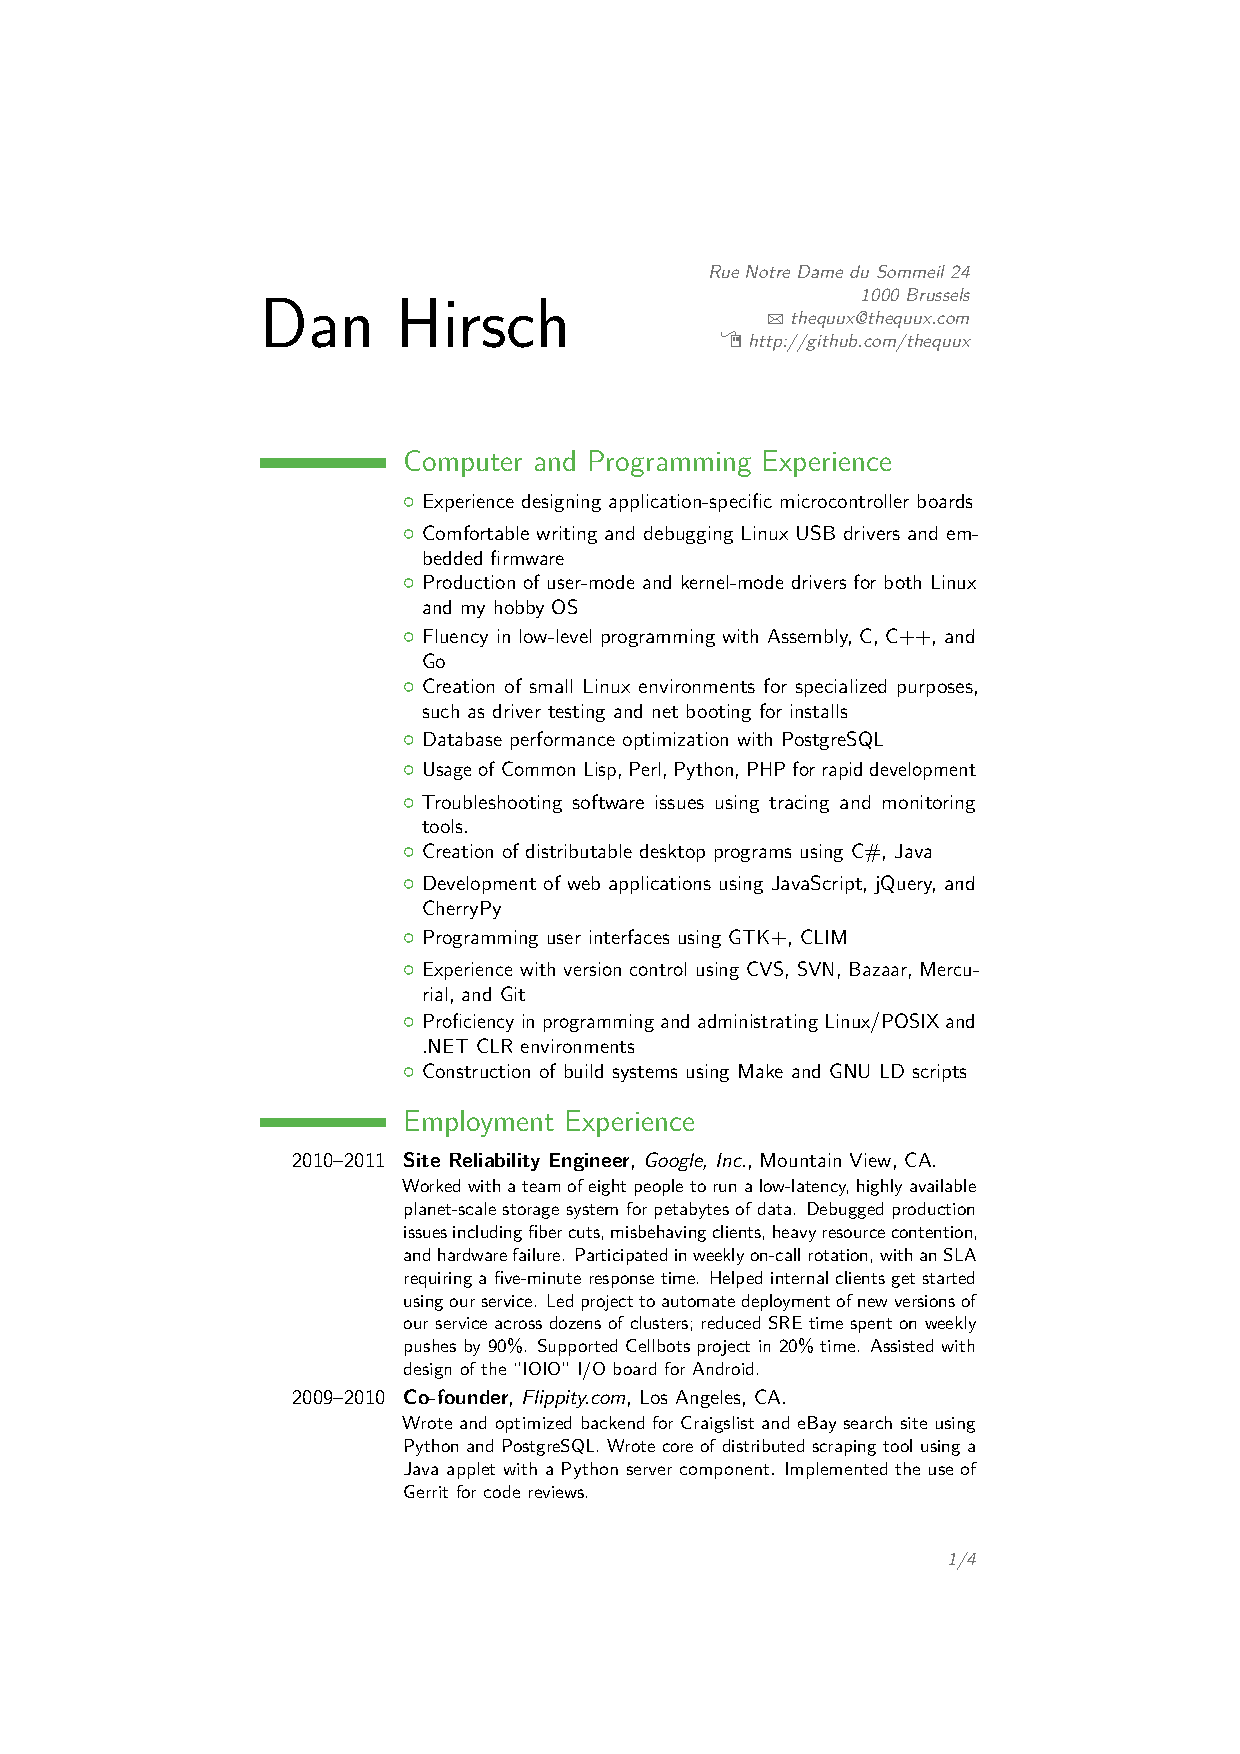
\includepdf[pages=-]{resumes/Hirsch.pdf}
	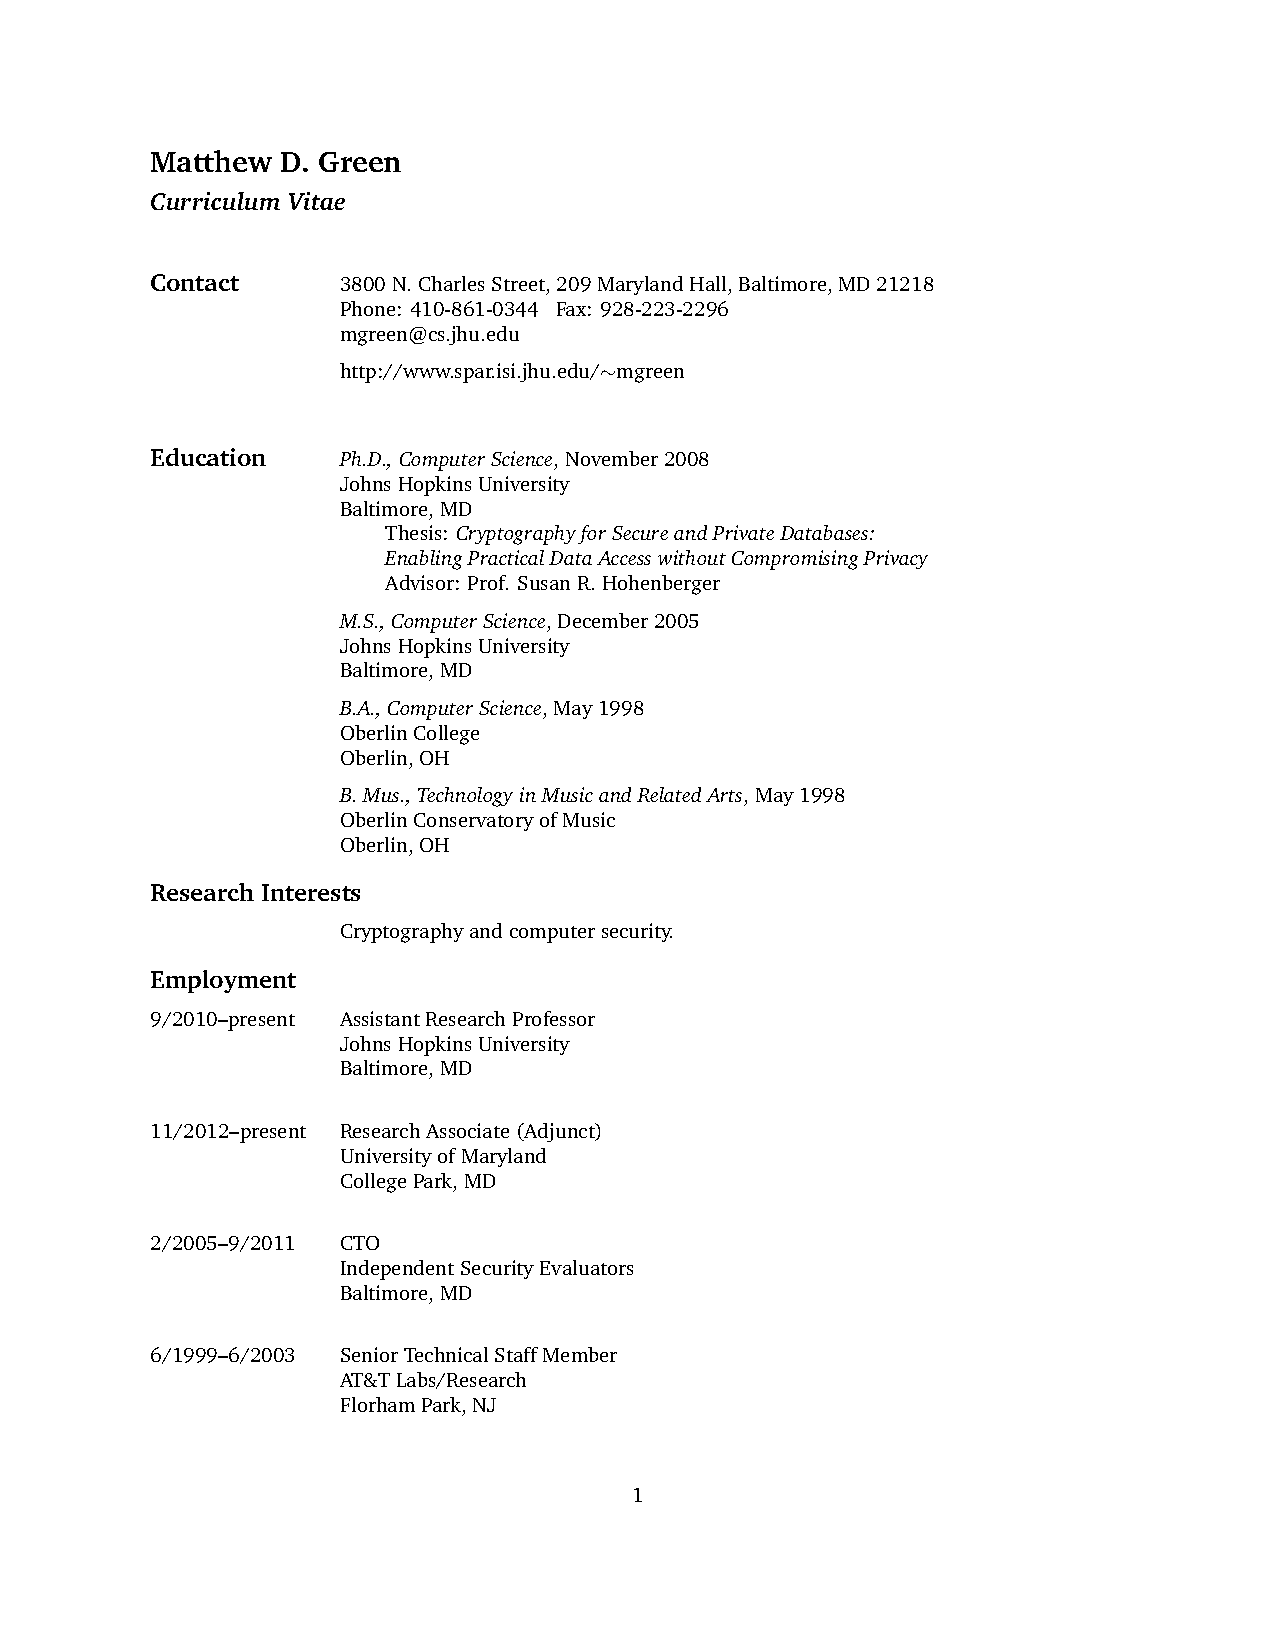
\includepdf[pages=-]{resumes/Green.pdf}
	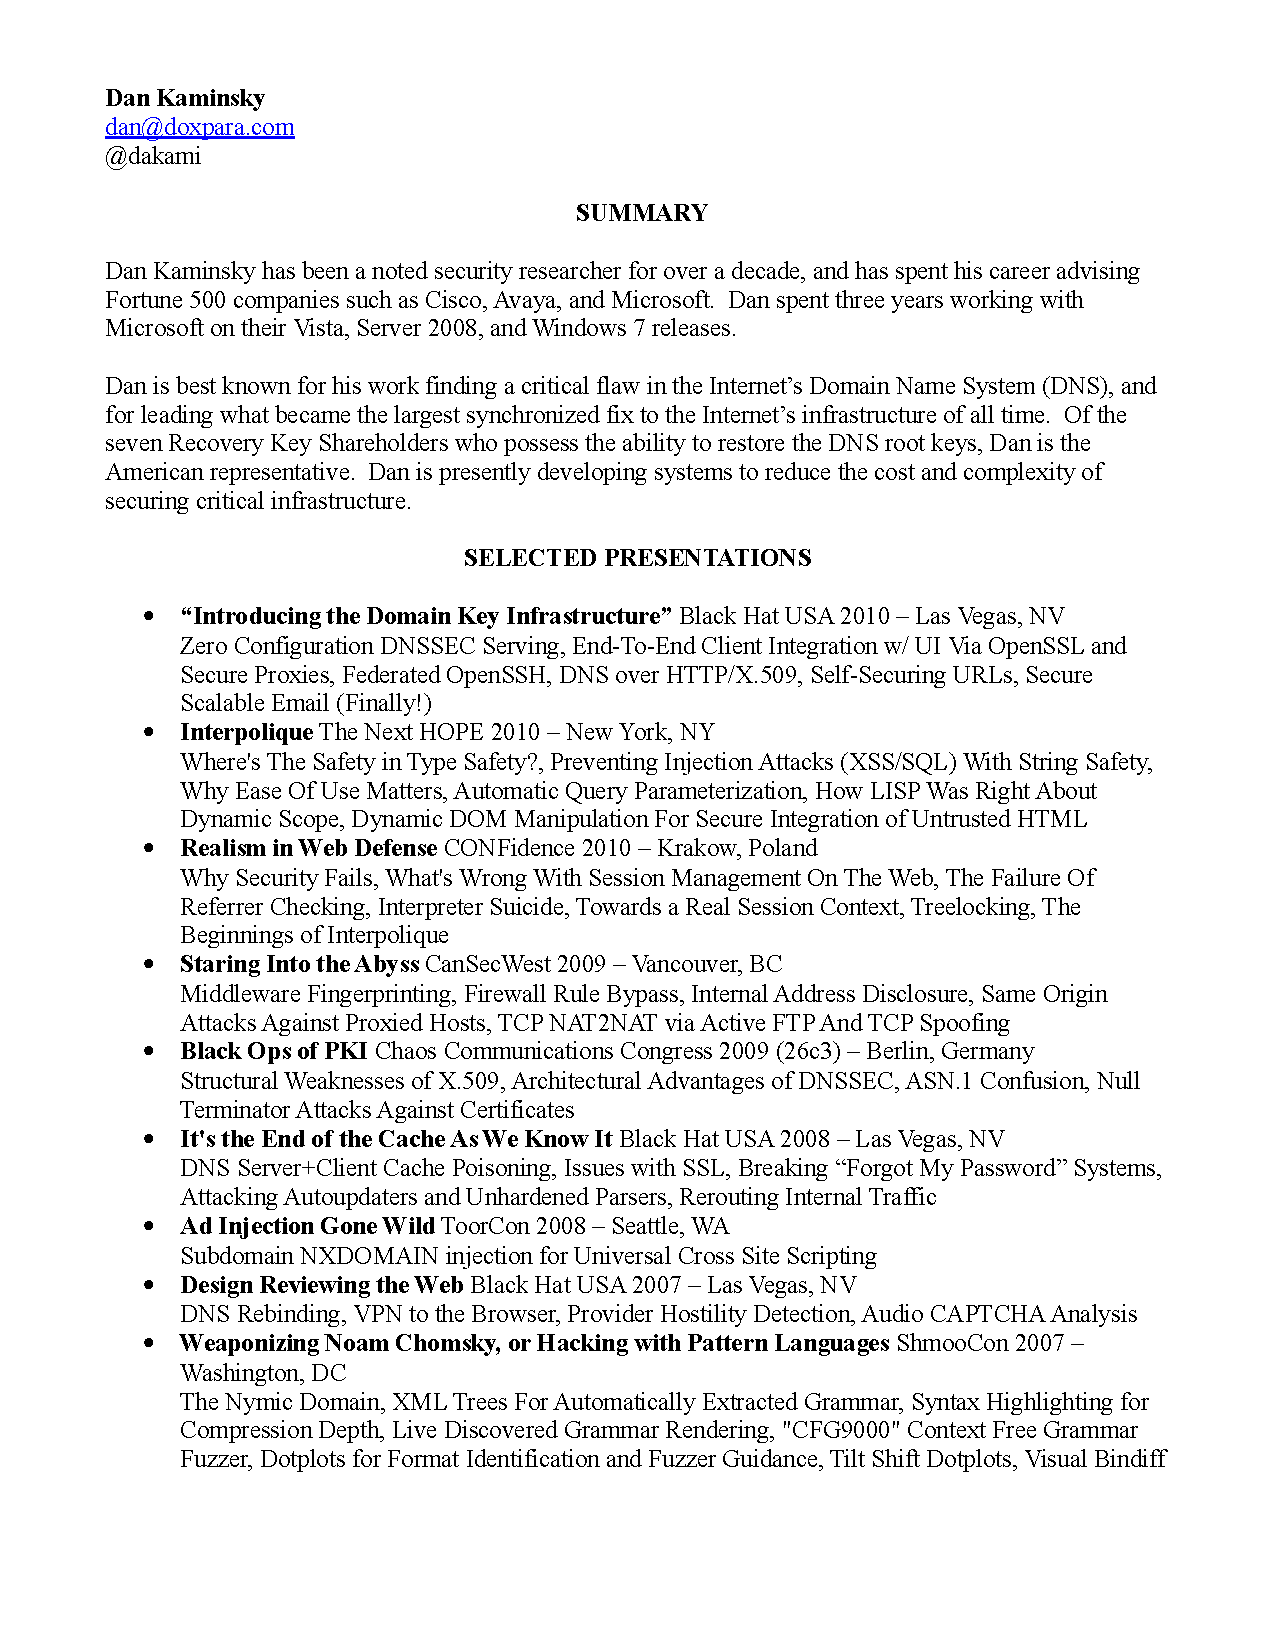
\includepdf[pages=-]{resumes/Kaminsky.pdf}
	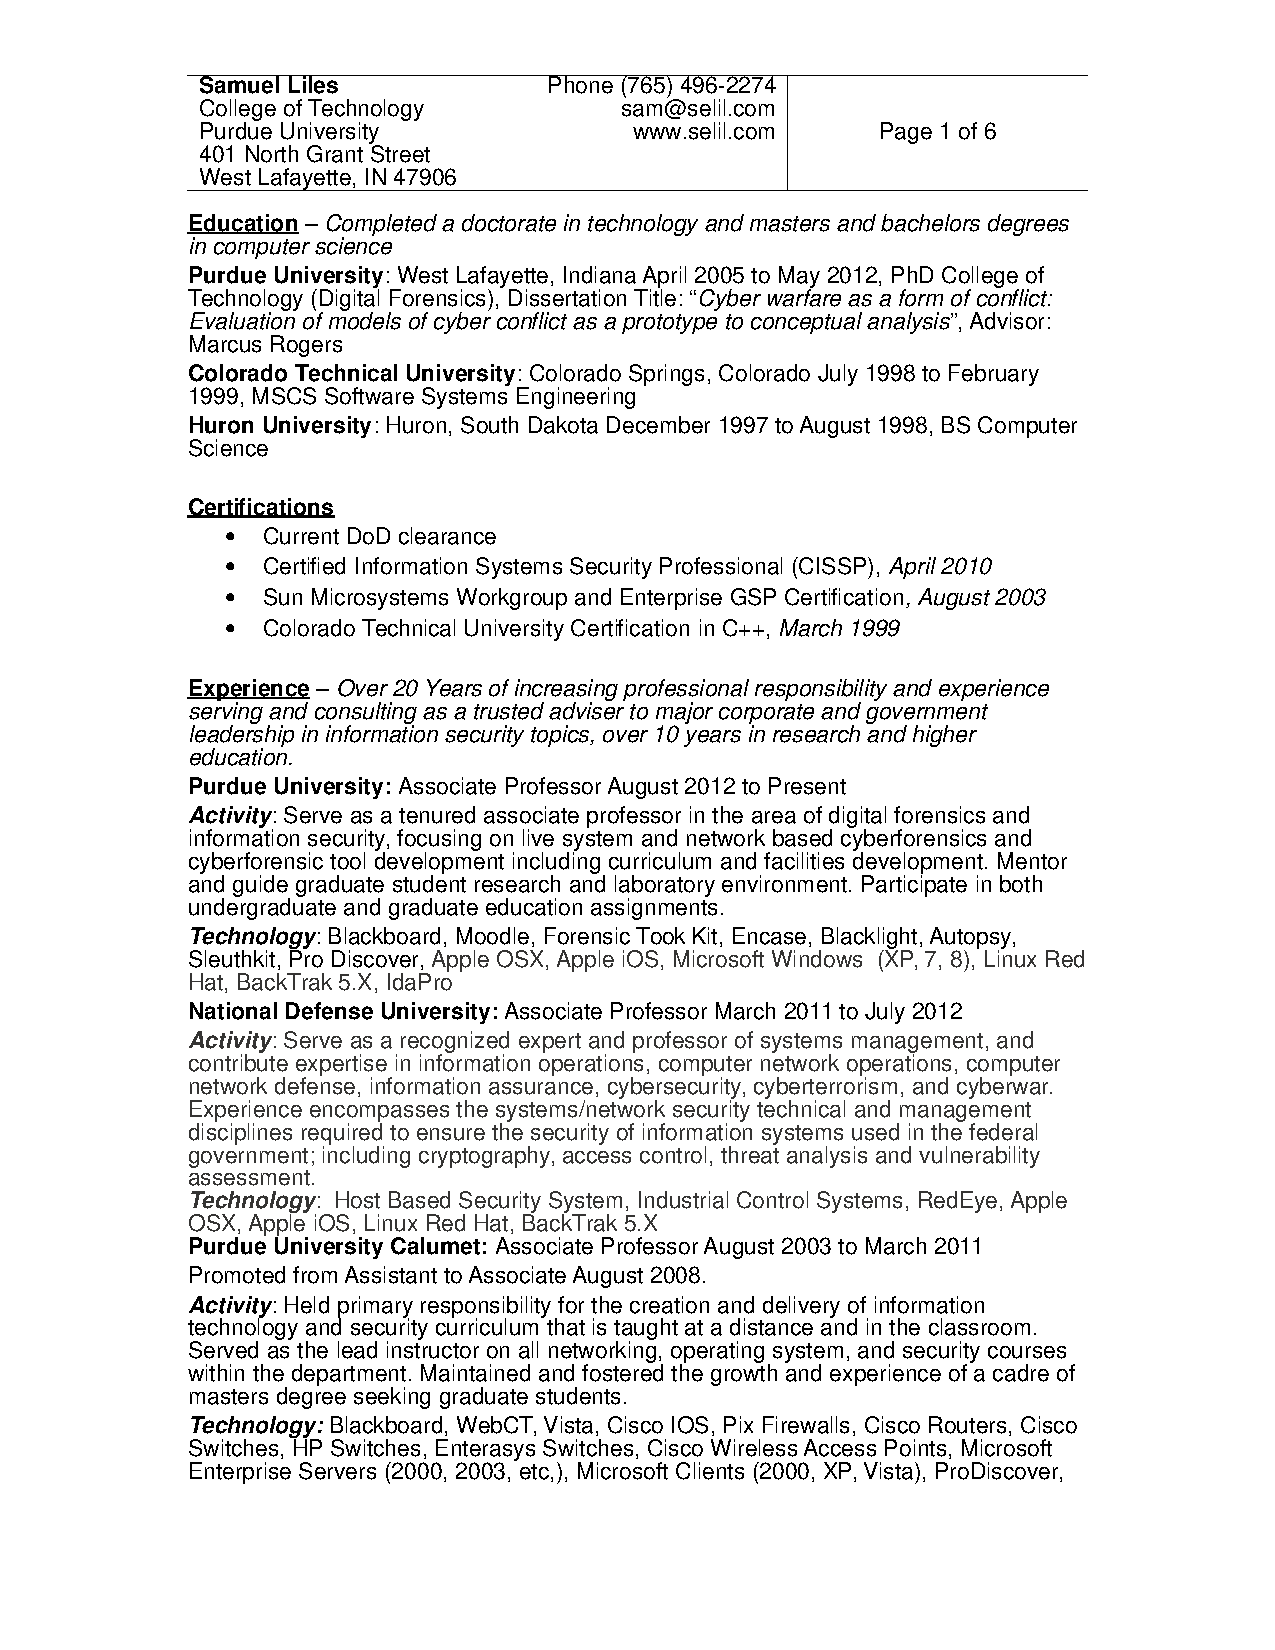
\includepdf[pages=-]{resumes/Liles.pdf}
	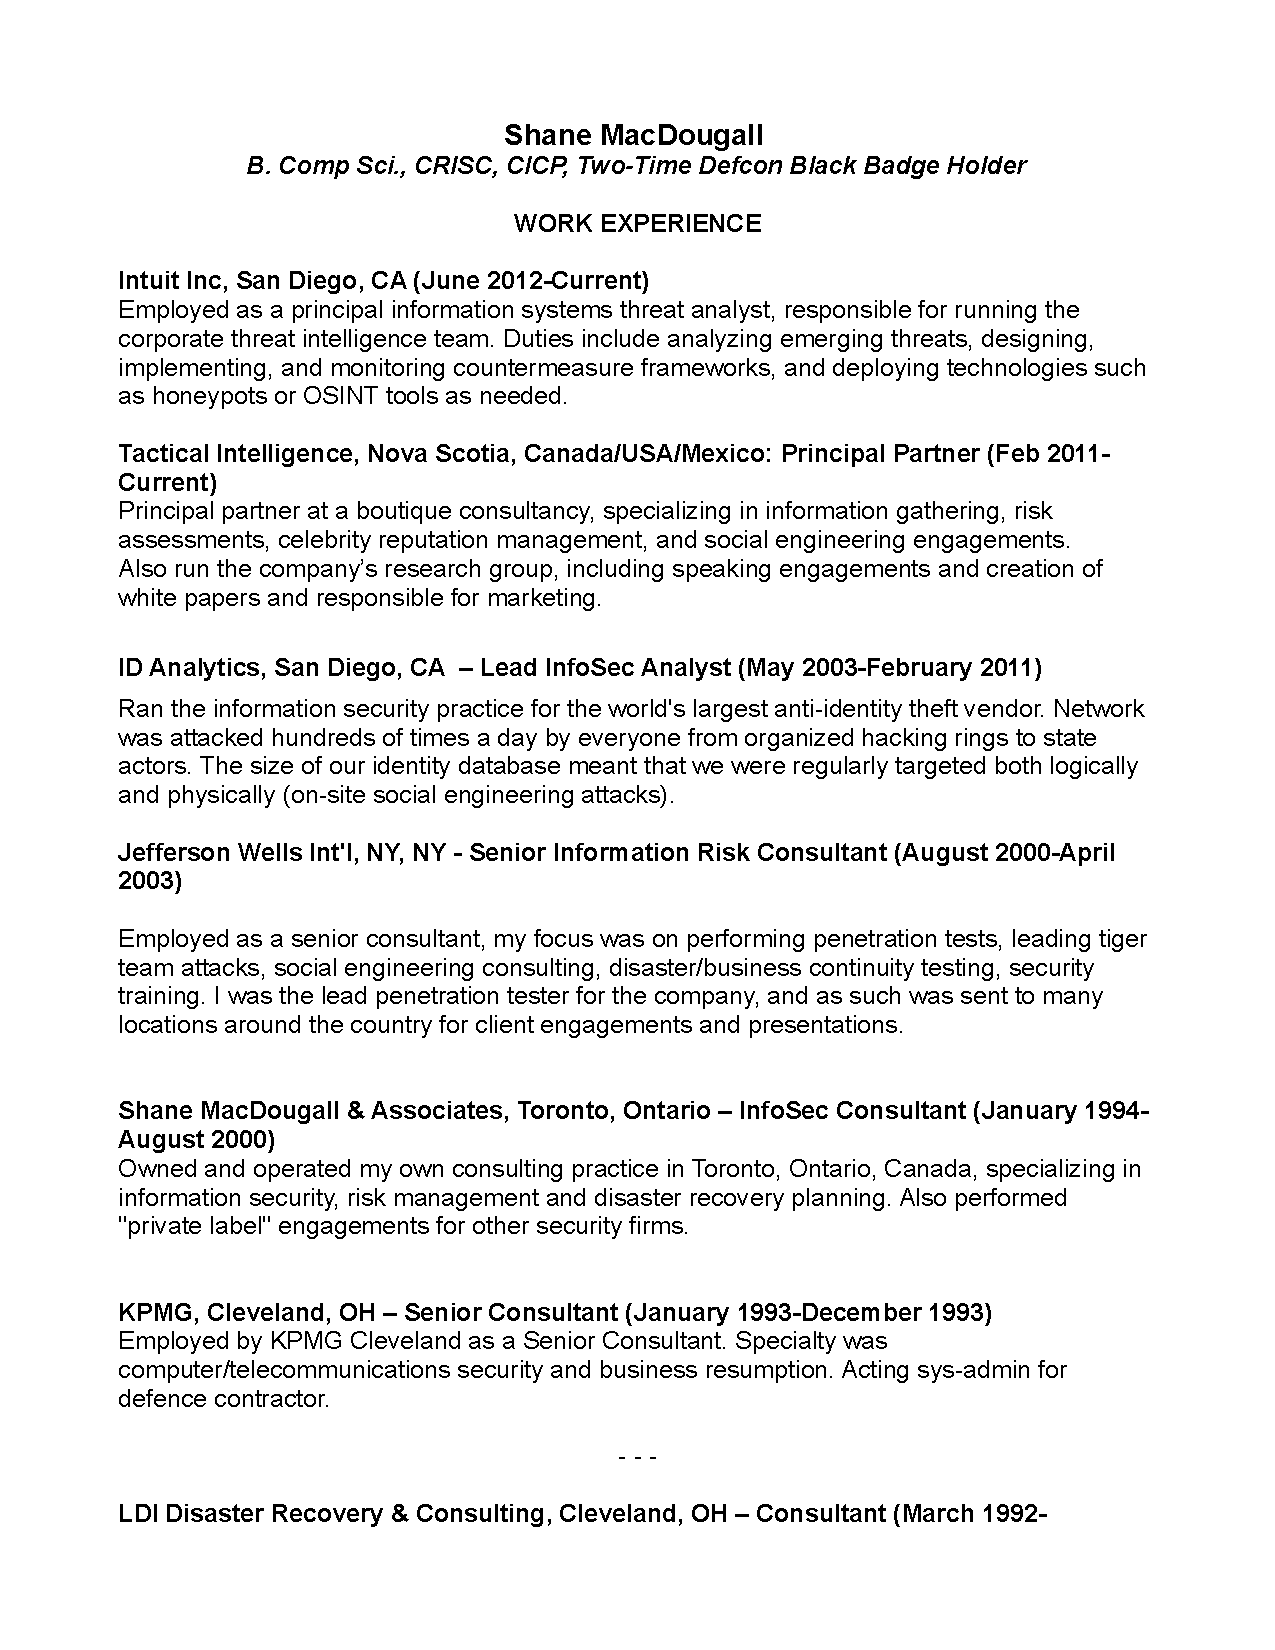
\includepdf[pages=-]{resumes/MacDougall.pdf}
	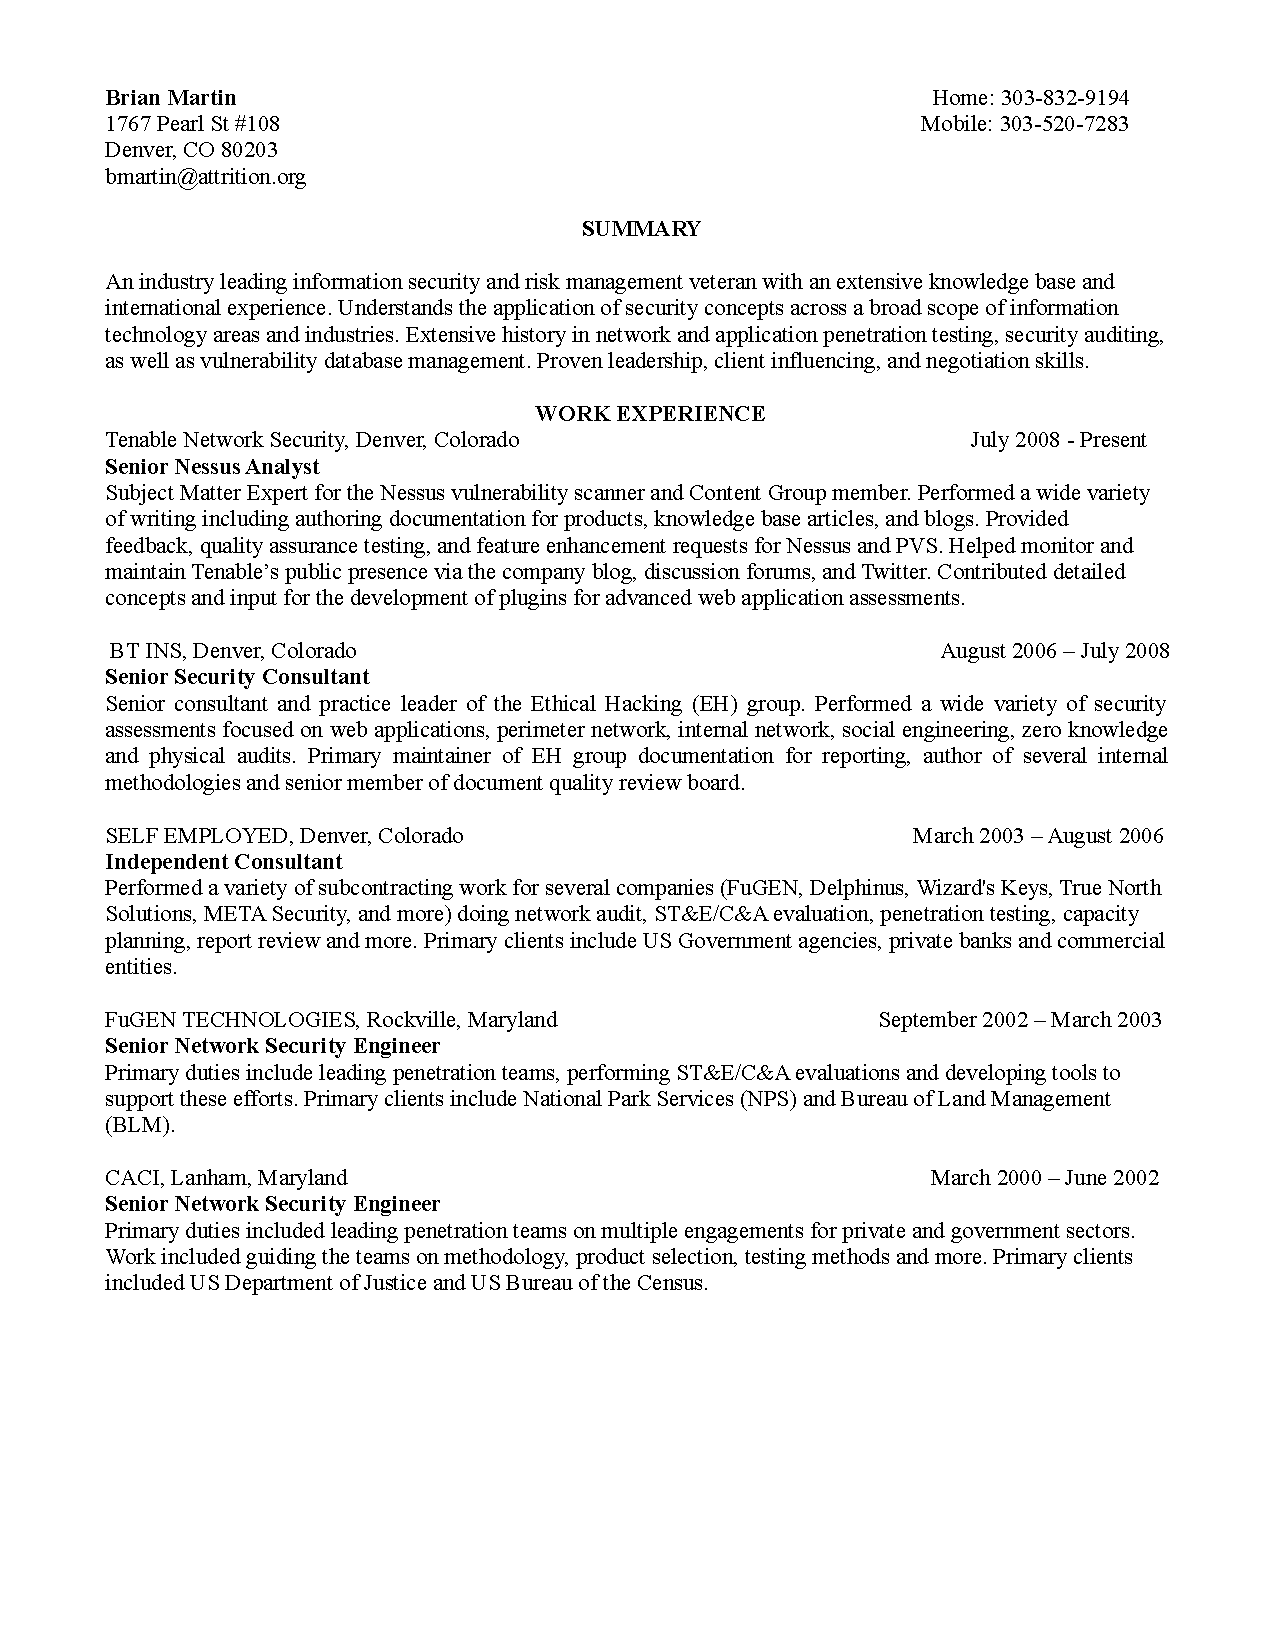
\includepdf[pages=-]{resumes/Martin.pdf}
	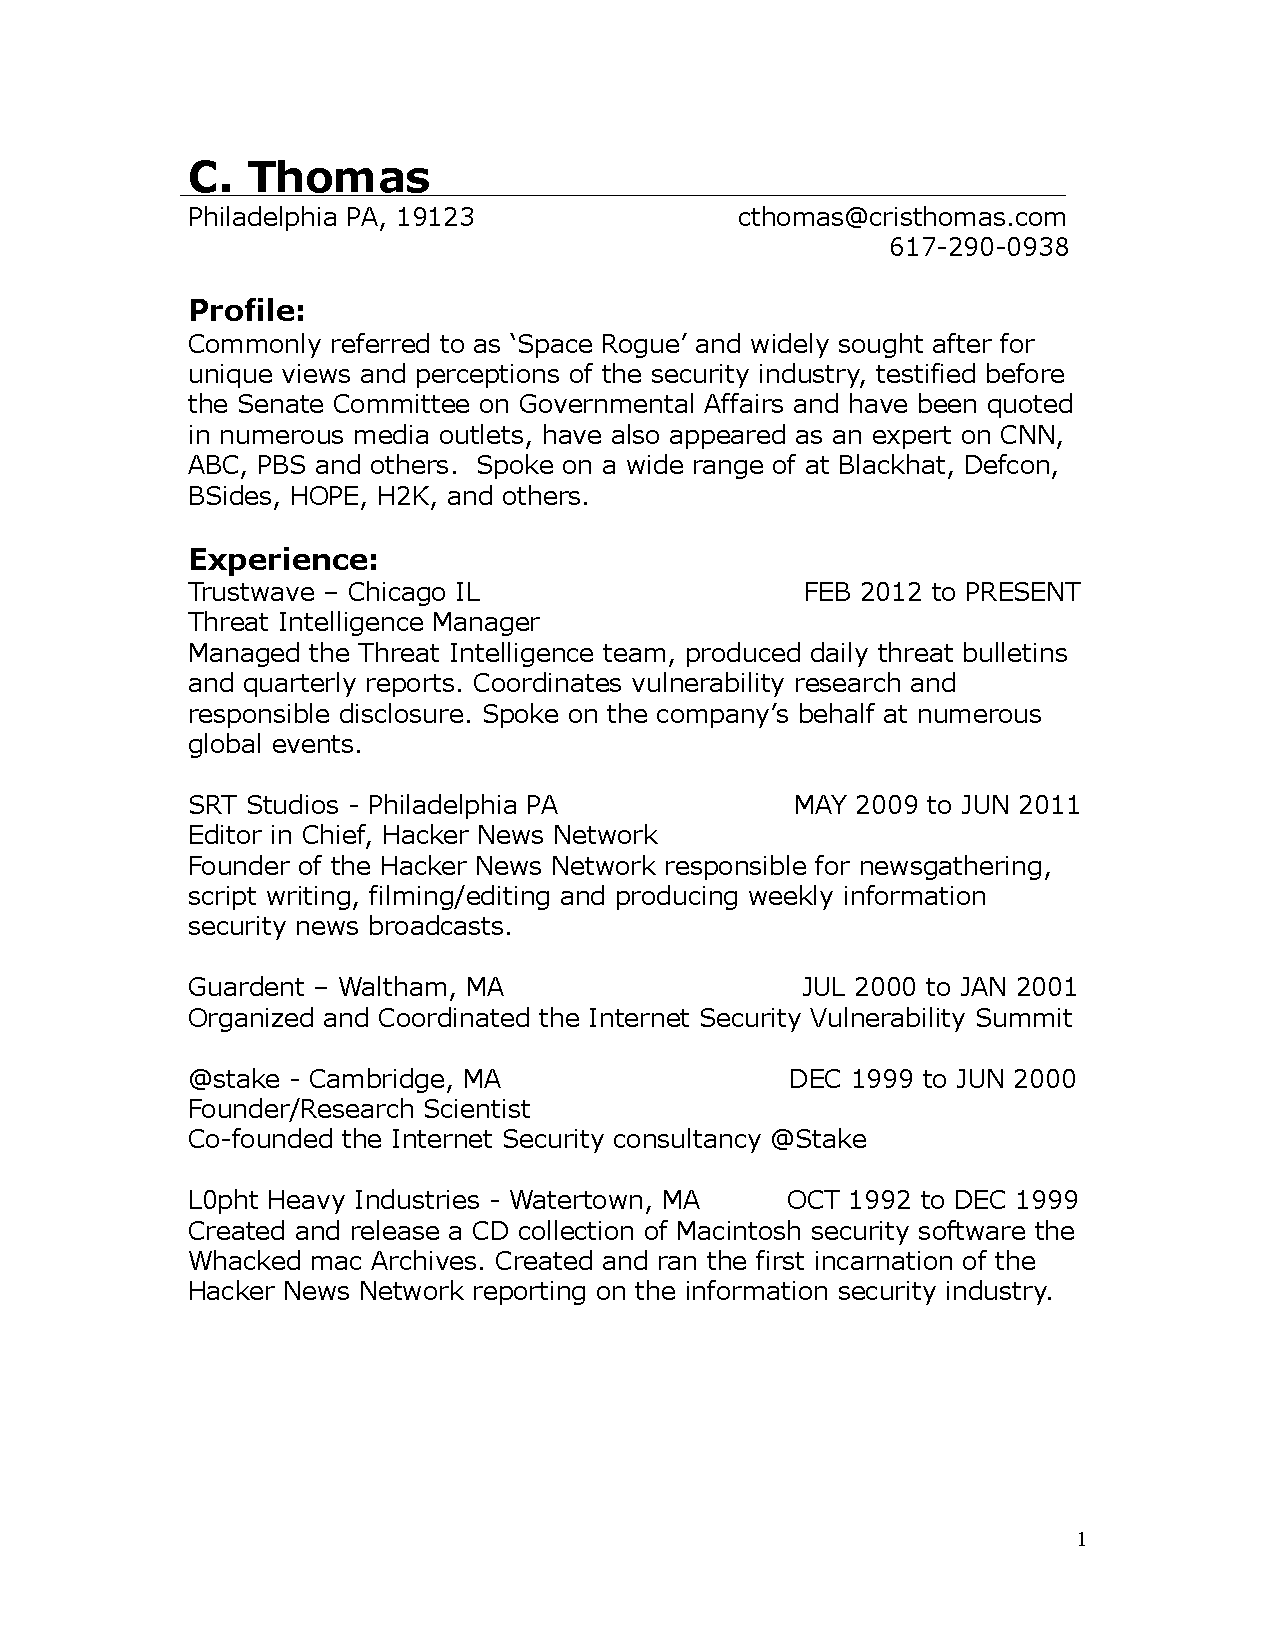
\includepdf[pages=-]{resumes/Thomas.pdf}
	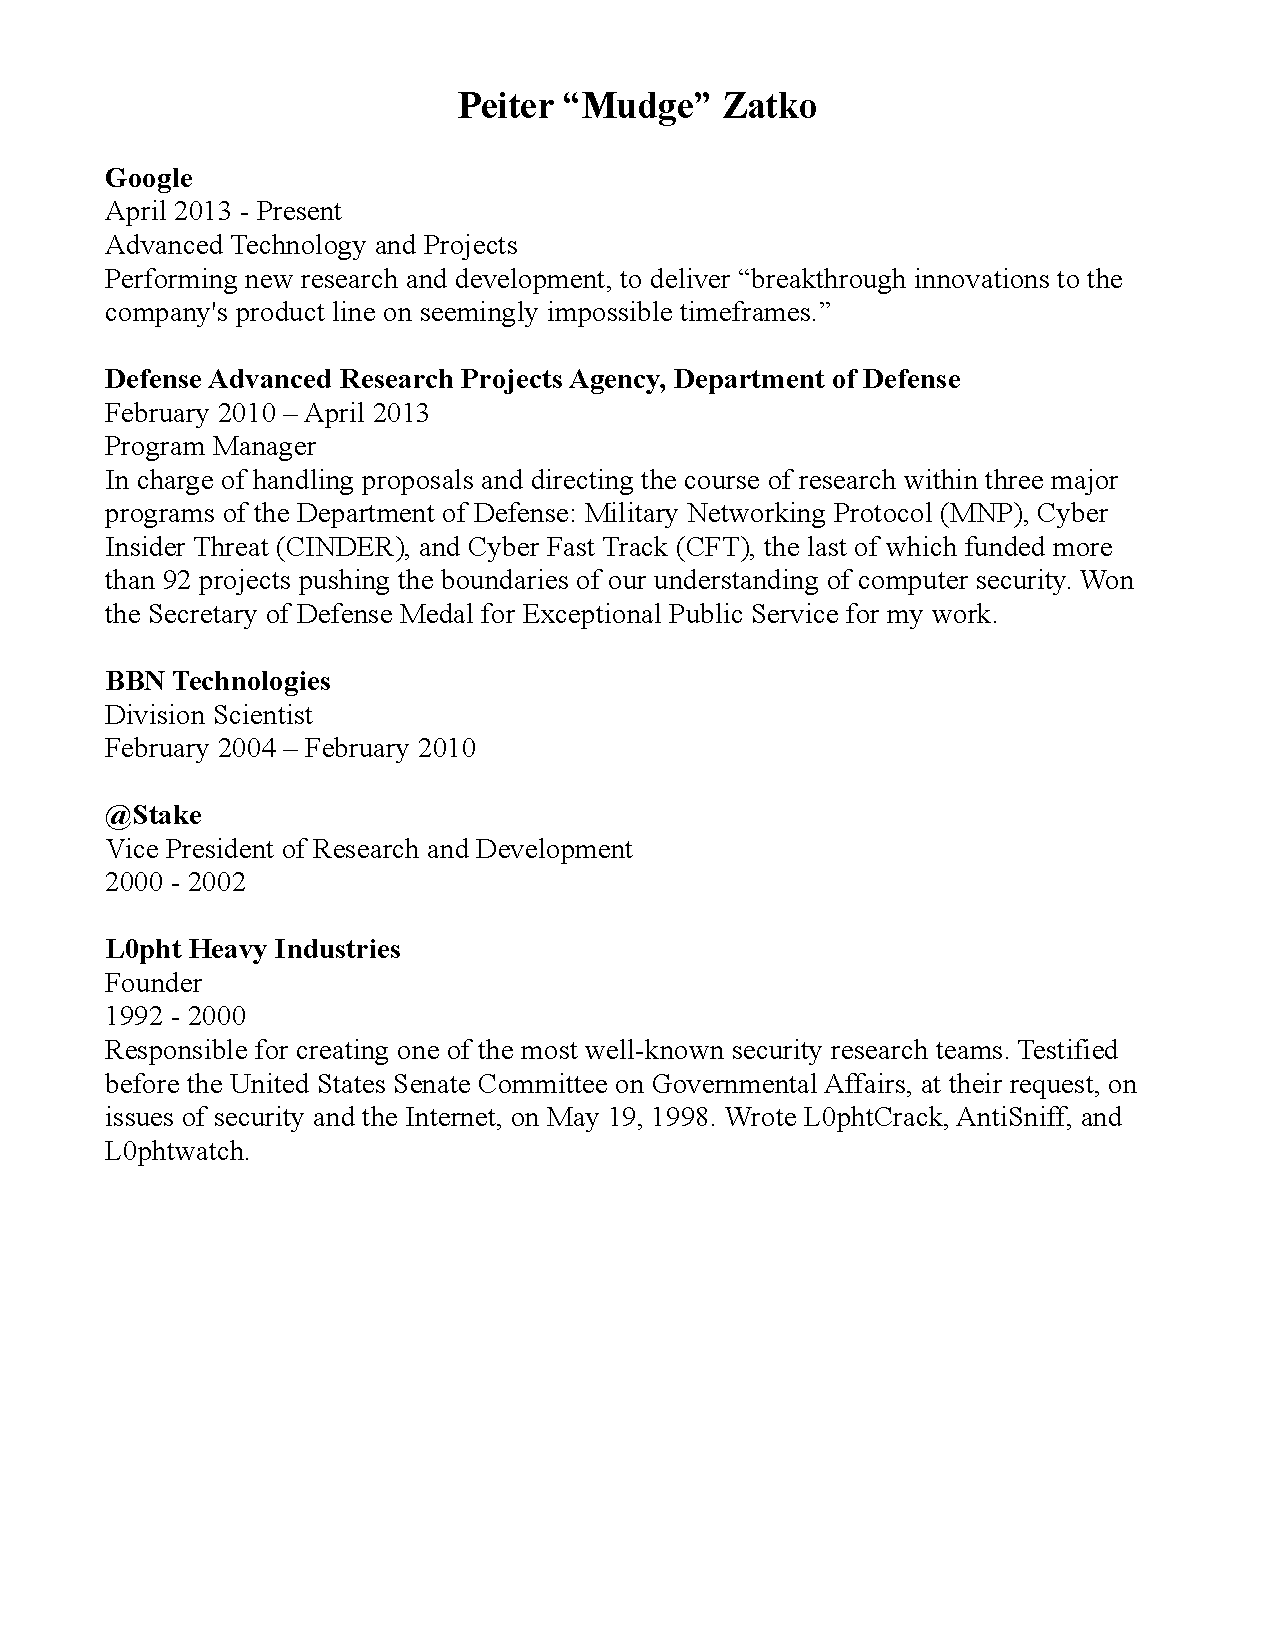
\includepdf[pages=-]{resumes/Zatko.pdf}
	
\end{document}
